\documentclass{article}

% NeurIPS 2026 style (official author kit: neurips_2026.sty, checklist.tex).
%   \usepackage{neurips_2026}            anonymous submission (Main Track): line numbers, no authors
%   \usepackage[preprint]{neurips_2026}  non-anonymous preprint, e.g. arXiv
%   \usepackage[main, final]{neurips_2026}  camera-ready, only after acceptance
% natbib is loaded by the style; pass its options before loading it.
\PassOptionsToPackage{numbers,compress}{natbib}
\usepackage{neurips_2026}

\usepackage[utf8]{inputenc}
\usepackage[T1]{fontenc}
\usepackage[hidelinks]{hyperref}
\usepackage{url}
\usepackage{booktabs}
\usepackage{amsmath,amssymb}
\usepackage{nicefrac}
\usepackage{microtype}
\usepackage{xcolor}
\usepackage{graphicx}
\graphicspath{{figures/}}
\usepackage{enumitem}

\usepackage{tikz}
\usetikzlibrary{shapes.geometric,arrows.meta,positioning,fit,calc,backgrounds}
\newdimen\pipelinewidth
\newdimen\trainwidth
\newdimen\valwidth
\newdimen\testwidth
\newdimen\barx
\newdimen\bary
\newdimen\sigx
\newdimen\sigy

\title{Uncertainty-Aware Machine Learning for Long-Term Neural Recordings in Flexible Brain-Computer Interfaces}

\author{%
  Guilherme Grancho Duarte Fernandes \\
  Imperial College London \\
  \texttt{guilherme.fernandes25@imperial.ac.uk} \\
}

\begin{document}

\maketitle

\begin{abstract}
A major challenge for the lasting reliability of brain-computer interfaces in real world conditions is neural drift, which degrades decoder performance and makes them unreliable over time. To evaluate the decline in accuracy, it's necessary to have recent labeled data, which is expensive and impractical in real life settings. This paper studies a learned class-conditional split-conformal layer to measure uncertainty in neural decoding models, without requiring new labeled data. A behavior-constrained variational autoencoder and a Transformer alignment decoder predict the maze region occupied by a mouse, then the conformal layer outputs a trust region of plausible maze regions. The approach was tested using electrophysiological data from flexible brain probes in 13 mice as they went through 3 virtual-reality mazes. For a targeted 90\% trust region accuracy, the method achieved 81.4\% to 86.5\% test accuracy when constructing trust regions that included the true maze region. The trust region size correlated positively with decoder error in two of the three mazes and negatively in the third. These results show that the proposed model gives a signal for decoding uncertainty, which is promising for long-term reliability in brain-computer interfaces. Nevertheless, a more thorough comparison with different methods and additional decoding models is necessary before broad implementation.
\end{abstract}

\section{Introduction}
Brain-computer interfaces (BCIs) predict behavior from neural activity using encoding-decoding pipelines~\cite{dong2023a}. In neural recordings, movements at the electrode and tissue point of contact, changes in the recorded neural population~\cite{tang2023a,vanbeest2025}, and alterations in neural representation~\cite{deitch2021,rule2019a} can modify the relationship between the neural activity and the predicted variable over time, causing neural drift. While alignment methods~\cite{karpowicz2025a,degenhart2020a} can improve decoder stability, they primarily improve accuracy. These methods do not measure the model uncertainty. Therefore, long-term neural decoding for real life BCI deployment needs not only accuracy, but also a trustworthy uncertainty signal that can be evaluated over time.

To assess an encoder-decoder's reliability, it is necessary to measure its performance on recently labeled data~\cite{karpowicz2024a}. However, obtaining labels at the point of use is impractical, and continuously retraining the entire model may not be feasible~\cite{fan2023a}.  This creates a gap between encoding-decoding accuracy measured during development and the reliability required during deployment~\cite{ovadia2019a}. Rather than trying to correct neural drift, this work aims to determine whether an uncertainty calibration method can show when decoder predictions become less reliable, without requiring new labeled data.

This paper proposes a learned class-conditional split-conformal layer added after the encoding-decoding pipeline~\cite{angelopoulos2022a}. For each neural input, after the decoder prediction, the conformal layer outputs a trust region set for that prediction. To create this, the conformal method targets a specific accuracy level for the trust region to contain the ground-truth, the target conformal level. The size of this trust set quantifies the trust region sharpness. As the trust region widens, its sharpness decreases, reflecting increased uncertainty in the encoding-decoding pipeline. Because calibration and test data may be impacted by neural drift, the central question is whether the calibrated conformal layer maintains a good coverage level and sharpness in the test data.

The presented method is studied using an existing encoding-decoding model that uses a behavior-constrained variational autoencoder (BC-VAE)~\cite{kingma2022a,pandarinath2018a} followed by a Transformer alignment decoder. This workflow maps neural electrophysiological data collected via a flexible brain probe~\cite{tang2023a,zhao2024} implanted in 13 mice who navigate 3 virtual-reality mazes to a prediction of which maze region the mouse is in. For each decoder’s output, the conformal layer is assessed as a reliability tool that creates a set of plausible maze regions, the trust region set, for a targeted conformal level.

The rest of the paper first gives extra context on long-term neural decoding and conformal uncertainty calibration. It then explains the experimental protocol, defines the conformal model, analyses the conformal performance, and discusses the limitations and implications of the proposed approach for BCI applications.

\section{Related Work}

\subsection{Changes in neural recordings}
Both recording instability and representational drift can degrade neural encoding and decoding. Recording instability affects which neural signals are collected and how. This might happen due to brain probe movement~\cite{tang2023a,steinmetz2021} and neural tissue response to the probe. Flexible probes, like those used in this study, can help reduce the physical mismatch between the sensor and the neural tissue, but they do not prevent representational drift. Because representational drift is a biological phenomenon that alters the relationship between the received information and the neural activity, meaning that the same stimulus can start being encoded in a different form in the brain as time advances~\cite{deitch2021,rule2019a}. Recording instability and representational drift can occur together, and it's almost unfeasible to distinguish their influence in the neural recordings. Therefore, in this paper, the term neural drift is used to refer to their combined effect.

\subsection{Alignment methods for decoding}
Alignment methods address neural drift by trying to preserve decoder accuracy. In order to do that, these techniques map neural activity from later recordings into a latent space representation compatible with the one the encoder has previously learned~\cite {karpowicz2025a,degenhart2020a}. This approach matters because it shows that useful decoding remains possible under neural drift and motivates the Transformer alignment decoder used in this paper. However, sustaining accuracy and reporting reliability are different problems. A decoder may still return a seemingly confident prediction even as its uncertainty increases, so an additional calibration layer is needed to determine when the prediction should be interpreted as unreliable~\cite{guo2017a,weiWeiGanChao2024}.

\subsection{Conformal classification}
Uncertainty calibration methods assess whether the model's confidence is correctly reflected in its predictions. One version of these methods is conformal classification, which converts predictions into scores~\cite{angelopoulos2022a,liang2026a}. Those scores then create a trust region that aims to contain the true data label a certain percentage of the time, the targeted coverage level. Therefore, conformal performance is measured by coverage and sharpness. Coverage quantifies how often the trust region contains the true label. Sharpness reflects the trust region's narrowness. In classification tasks on imbalanced datasets, conformal methods can perform poorly for rare classes in the dataset, motivating the class-conditional conformal approach used in this paper, fully described in Section~\ref{sec:class-conditional}.

The reliability of conformal methods depends on the relationship between the calibration and test data. This is especially important in long-term neural recordings, where neural drift can cause later test data points to mean something else from earlier calibration ones. So, an evaluation method that tries to simulate a deployment scenario should therefore split calibration data from test data, using a split-conformal methodology~\cite{angelopoulos2022a}. Finally, by combining the class-conditional and split-conformal approaches,  the proposed solution is created, a class-conditional split-conformal layer for BCI applications to quantitatively assess the impact of neural drift.

\section{Experimental Setup}

\subsection{Data collection}
The dataset used in this paper is from extracellular neural spike recordings from the visual and motor cortices, detecting the electrical activity of neurons outside the cell membrane. These were collected using flexible brain probes implanted in 13 mice as they went through 3 different virtual reality mazes: the Linear Maze, the Y Maze, and the Loop Maze. In this setup, the mice faced 6 monitors and explored the mazes using an omnidirectional ball connected to the virtual environments, receiving water through a robotic arm as a reward when they reached maze checkpoints (Figure~\ref{fig:data-input}). The maze configurations stayed consistent across recording sessions. However, the recorded neural population activity could change over time due to neural drift.

For each tracked neuron, the number of electrophysiological spike impulses that occurred in the last 100 ms is recorded, creating firing-rate bins expressed in Hertz at a 100 ms resolution. The firing-rate bins are then grouped into windows of 10 bins, also called spike-count windows. Providing the encoder with 1 s interval information over all recorded neurons for each input spike-count window. Each input is labeled with the maze region the mouse occupies at that time, producing the classification task for the decoder. Figure~\ref{fig:data-input} shows the data collection setup and a session’s data example.

\begin{figure}[t]
  \centering
  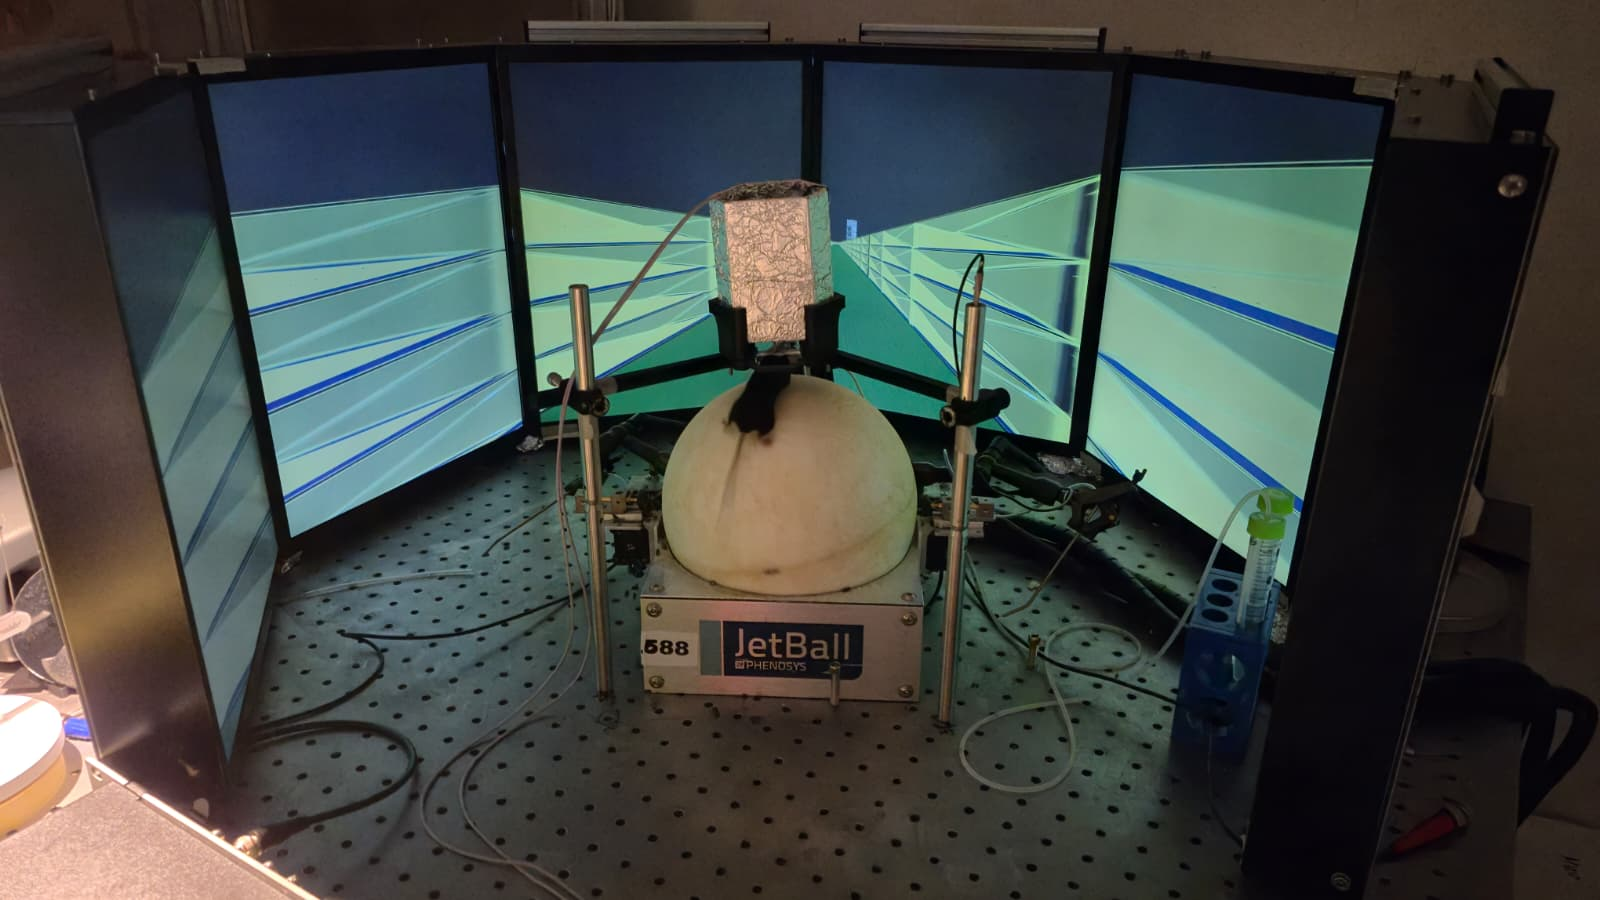
\includegraphics[width=0.45\linewidth]{set_up.jpeg}
  \hfill
  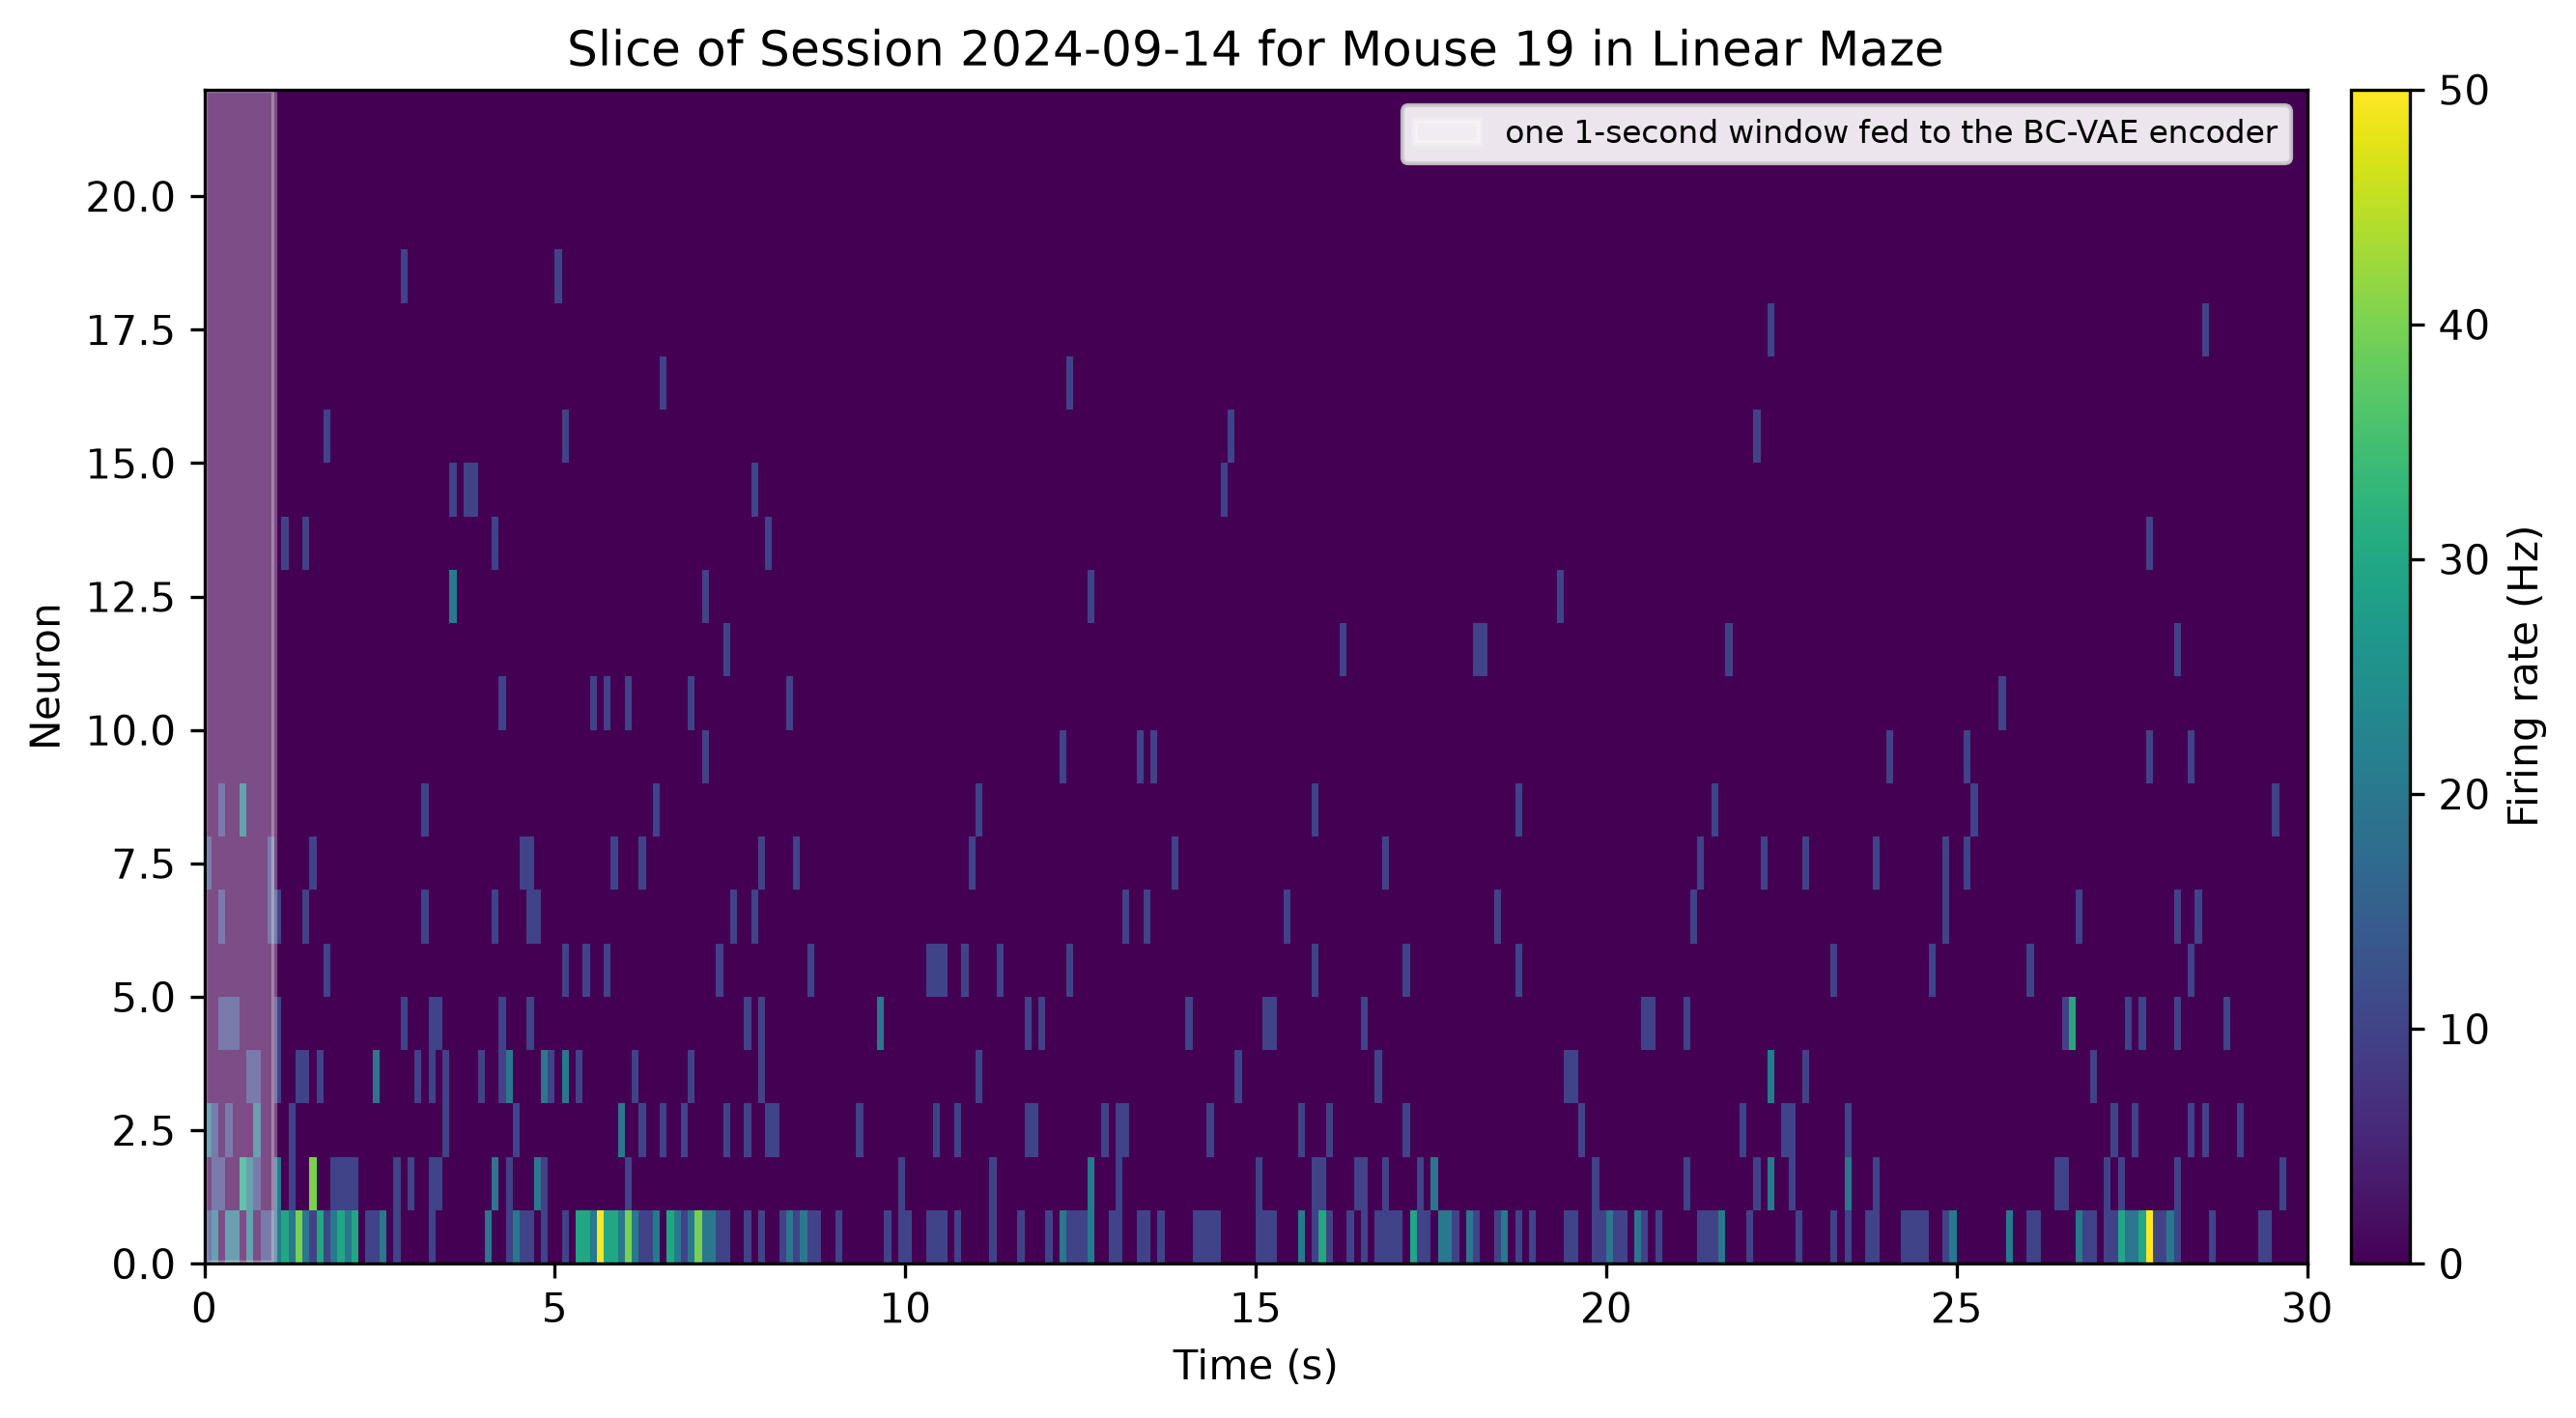
\includegraphics[width=0.47\linewidth]{encoder-input-example.png}
  \caption{Data collection and neural input. Left: Photograph of the Liu Lab's setup, which includes a mouse mounted on an omnidirectional ball, 6 monitors showing the maze environment, a flexible brain probe implanted in the animal, and an automated water delivery system. Right: The first 30 seconds of a Linear Maze session from Mouse 19 on 2024-09-18. The highlighted region corresponds to a 1 s interval input for the BC-VAE.}
  \label{fig:data-input}
\end{figure}

\subsection{Classification Task}
The dataset for each maze is created by aggregating the sessions for every mouse. Recording sessions with only one maze region label are removed to exclude failed sessions. The final dataset includes, for the Linear Maze, 13 mice and 95 sessions, for the Y Maze, 7 mice and 23 sessions, and for the Loop Maze, 2 mice and 14 sessions. Each session was split chronologically. The first 80\% of each session is combined across all sessions to create the training set. The next 10\% of each session is combined across all sessions to create the validation set, also used for the final calibration of the conformal layer. And the final 10\% of each session is combined across all sessions to create the test set.

For each maze, $\mathcal{Y}=\{1,\ldots,K\}$ is the set of possible maze region labels, illustrated in Figure~\ref{fig:maze-region}. Each neural input $x$ is labeled with a maze region $y\in\mathcal{Y}$. The encoder-decoder pipeline outputs region probabilities $\hat p_k(x)$ and the top prediction $\hat y(x)$. Afterwards, for each decoder prediction, the conformal layer creates a trust region set $\widehat{\mathcal{C}}(x)\subseteq\mathcal{Y}$. The conformal performance is evaluated by coverage and sharpness. Coverage is the frequency with which $y$ is inside $\widehat{\mathcal{C}}(x)$. Sharpness is the trust region size relative to the total number of maze regions, $|\widehat{\mathcal{C}}|/K$.

\begin{figure}[t]
  \centering
  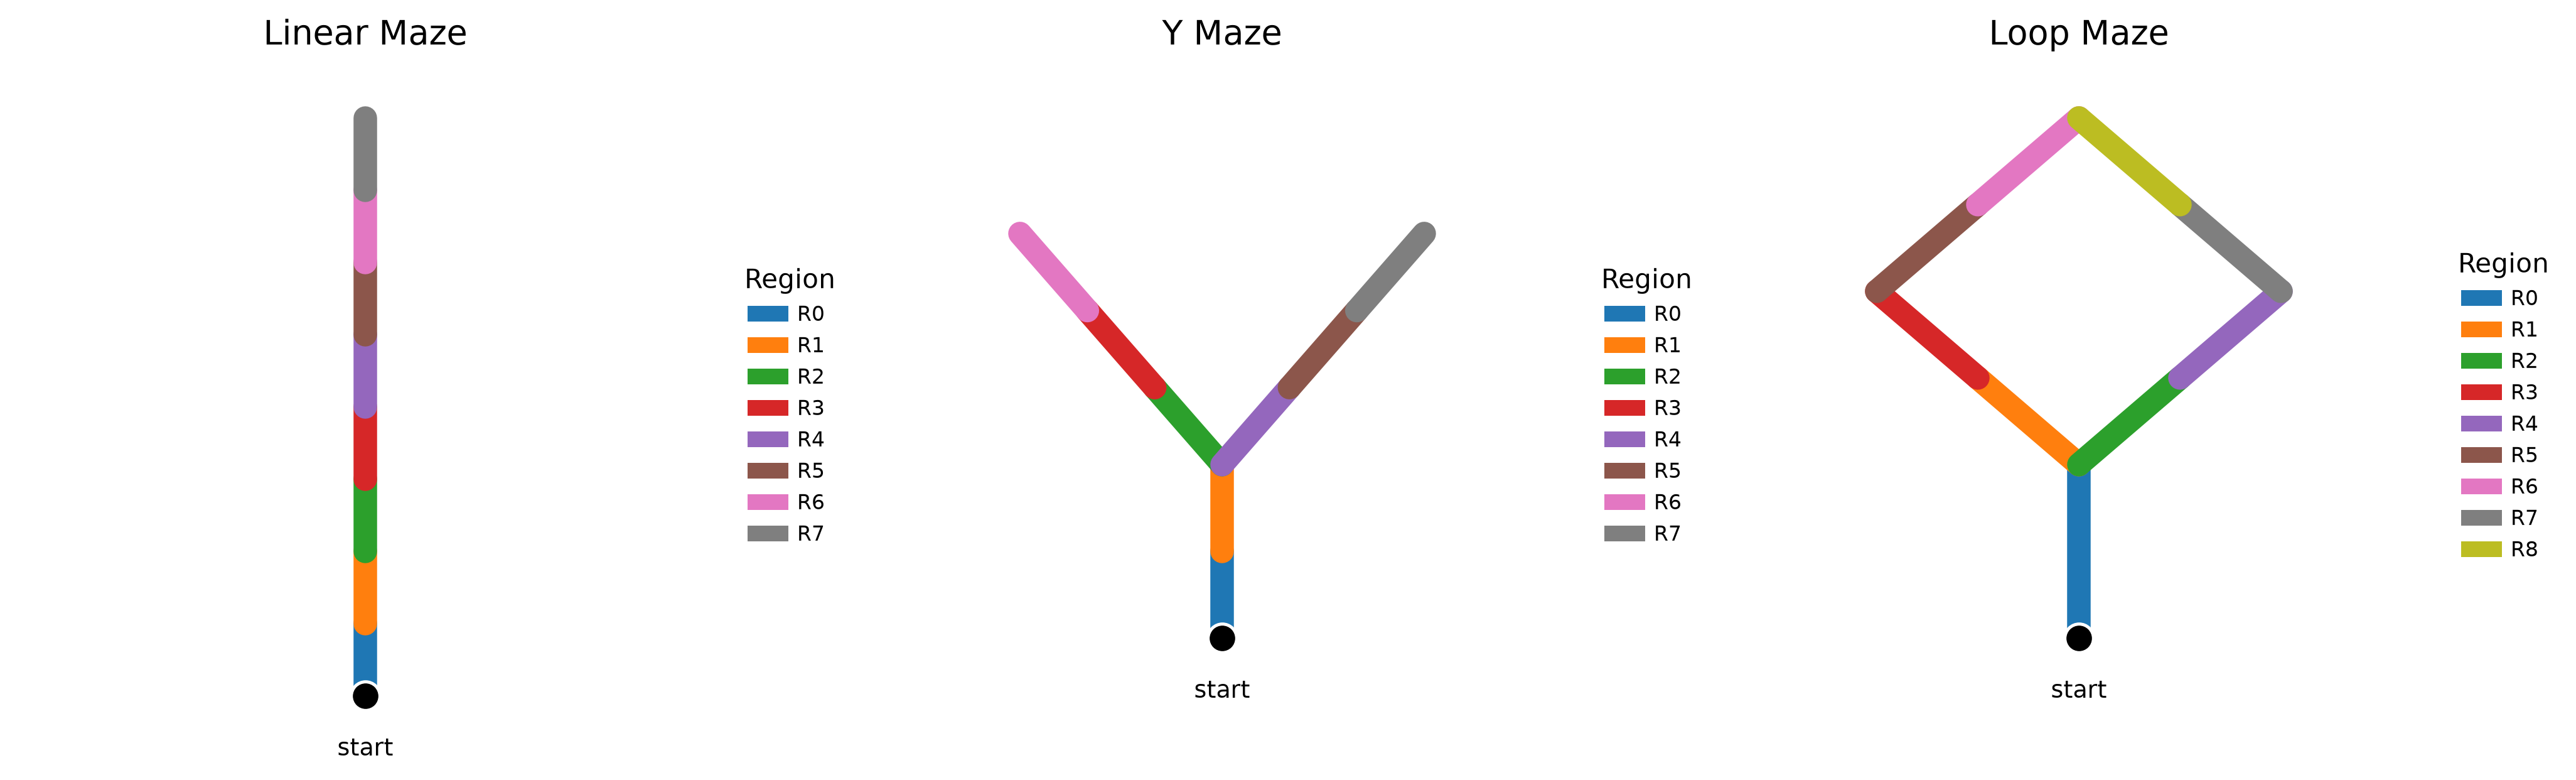
\includegraphics[width=0.99\linewidth]{maze-geometry.png}
  \caption{This schematic shows the 3 maze layouts with discrete region labels. The black dot marks the start of the trial.}
  \label{fig:maze-region}
\end{figure}

\subsection{Encoding-decoding pipeline}
The encoding-decoding workflow consists of a BC-VAE followed by a Transformer alignment decoder. For each spike-count input window, the BC-VAE produces a latent space represented by a mean and a variance. The Transformer processes a sequence of 5 latent means from the BC-VAE and outputs a probability distribution over the maze regions, from which the top probability is the final decoder prediction. The conformal layer studied in this paper is applied after this decoder. Decoder accuracy is therefore reported as extra context for the conformal analysis, while the main focus is the coverage and sharpness of the proposed conformal approach.

\subsubsection{BC-VAE}
The BC-VAE is initialized with a Gaussian prior latent space with 16 dimensions $\mathcal{N}(0,I)$~\cite{kingma2022a}. As spike-count windows $x$ start being inputted, the encoder maps them into the posterior latent space $z$ parameterized by a posterior mean vector $\mu(x)\in\mathbb{R}^{16}$ and a posterior variance vector $\sigma^2(x)\in\mathbb{R}^{16}$. In the implementation, the encoder outputs the variance on a logarithmic scale, which is converted back to a regular scale when required. The model is trained to encode the spike counts~\cite{pandarinath2018a} in a posterior latent space that is regularized towards the normal prior $\mathcal{N}(0,I)$~\cite{higgins2017a}, while preserving the maze region information in the new latent representation. After training, $\mu(x)$ serves as the latent representation passed to the Transformer decoder, while $\sigma^2(x)$ is used as an uncertainty signal for the conformal layer.

\subsubsection{Transformer alignment decoder}
As an alignment strategy to improve decoding performance, a Transformer alignment decoder processes a sequence of 5 consecutive BC-VAE posterior mean vectors $\mu(x)$. So, for a prediction at $t$, the input is $(\mu_{t-4},\ldots,\mu_t)$. If fewer than 5 vectors are available at the start of a session, the first mean vector is repeated as needed. During training, the model tries to align and closely represent the same maze region in the new aligned latent space across different sessions and animals~\cite{schneider2023a}, to gain generalizability across mice and sessions, while fighting neural drift. Finally, from the new latent representation, a softmax probability vector $\hat p(x)$ over the maze regions is inferred. The decoder’s final maze region prediction $\hat y(x)$ is the highest value in the probability vector $\hat p(x)$.

\subsection{Uncertainty signals}
\label{sec:uncertainty-signals}
To learn to quantify the system's uncertainty, the conformal layer receives 4 uncertainty signals per input: the BC-VAE posterior variance, the encoder Jacobian norm, the alignment Jacobian norm, and the predictive entropy.

\subsubsection{BC-VAE posterior variance}
The BC-VAE posterior variance uncertainty signal reduces the encoder's variance vector output with 16 dimensions $\sigma^2(x)$, to a single scalar $\bar{\nu}$ for each spike-count window $x$. Considering that, $\sigma^2_j(x)$ is the scalar posterior variance assigned to the latent dimension $j$. The variance signal is the mean across all latent dimensions:

\begin{equation}
  \bar{\nu}=\frac{1}{d}\sum_{j=1}^{d}\sigma_j^2(x), \qquad d=16.
\end{equation}

A larger mean posterior variance indicates that the encoder assigns higher uncertainty to the current spike-count window latent representation before Transformer decoding.

\subsubsection{Encoder Jacobian norm}
The encoder Jacobian norm measures the largest impact that perturbations on the input $x$ can have on the BC-VAE posterior mean output $\mu(x)$~\cite{barter2019a,miyato2018a}. For each window $x$, the signal is defined as the spectral norm of the derivative from the input window to the latent mean with 16 dimensions:

\begin{equation}
  \mathcal{J}^{\mathrm{enc}}
  =\left\lVert\frac{\partial \mu(x)}{\partial x}\right\rVert_2 .
\end{equation}

This scalar is the largest singular value, indicating the greatest encoder sensitivity. Larger values mean greater response to small input modifications.

\subsubsection{Alignment Jacobian norm}
The alignment Jacobian spectral norm measures sensitivity at the Transformer alignment stage~\cite{barter2019a,miyato2018a}. Considering that, $f$ is the Transformer model that receives a sequence of 5 BC-VAE posterior means to output the aligned latent representation. For window $x_t$, the signal measures the derivative of the aligned latent space with respect to the current latent mean $\mu(x_t)$:

\begin{equation}
  \mathcal{J}^{\mathrm{align}}_t
  =\left\lVert
  \frac{\partial f(\mu(x_{t-4}),\ldots,\mu(x_t))}
  {\partial \mu(x_t)}
  \right\rVert_2 .
\end{equation}

Like the encoder Jacobian, this value is the largest singular value of the derivative. Higher values mean small changes in the BC-VAE latent mean lead to larger changes in the Transformer latent representation.

\subsubsection{Predictive entropy}
This signal is computed as the entropy of the decoder's softmax output $\hat p(x)$ over the $K$ maze regions~\cite{lakshminarayanan2017a}. This entropy summarizes the uncertainty of the full $\hat p(x)$ vector distribution over all possible $k$ labels:

\begin{equation}
  \mathcal{H}=-\sum_{k=1}^{K}\hat p_k(x)\log \hat p_k(x).
\end{equation}

Entropy is zero when all probability is assigned to one region and is the largest for a uniform distribution over all regions. It therefore captures global ambiguity in the decoder output.

\subsection{Learned class-conditional split-conformal layer}
The learned class-conditional split-conformal layer is applied after training the encoding-decoding pipeline. It uses the 4 uncertainty signals from Section~\ref{sec:uncertainty-signals} to learn a positive scale factor that indirectly adjusts the trust region size to achieve a targeted coverage level.

\subsubsection{Learned uncertainty scale}
The 4 uncertainty signals, from Section~\ref{sec:uncertainty-signals}, are combined into a vector $u(x)\in\mathbb{R}^{4}$. This vector $u(x)$ is given as input to a multilayer perceptron (MLP) composed of 4 input neurons for each uncertainty signal, 2 layers each with 32 neurons, and a final single output neuron. This tiny MLP outputs $\sigma_\theta(x)$ as one positive value for each spike-count window. Not to be confused with the variance of the BC-VAE $\sigma^2(x)$, the MLP output notation uses $\theta$. With this, $\sigma_\theta(x)$ becomes the main final uncertainty signal used throughout the rest of the conformal layer. The MLP loss function is described in Section~\ref{sec:conformal-loss}.

\subsubsection{Scaled conformal scores}
For each maze region $k$, the scaled conformal score is defined as:

\begin{equation}
  S(x,k)=\frac{1-\hat p_k(x)}{\sigma_\theta(x)} .
\end{equation}

Maze regions that have lower scores $S(x,k)$ are more likely to be included in the trust region set. A lower numerator means the decoder is more confident in maze region $k$, producing a lower score and making it more likely for $k$ to be included in the trust region. A higher denominator means that the input $x$ produced higher uncertainty signals throughout the encoding-decoding pipeline, culminating in a higher $\sigma_\theta(x)$, lowering scores for all maze regions for that input $x$, relaxing the border of the trust region for that high uncertainty input $x$, and making the maze regions more likely to be included in the trust region. Concluding, both greater uncertainty $\sigma_\theta(x)$ and higher decoder probability $\hat p_k(x)$ result in a maze region $k$ being more likely to be part of the trust region. During conformal calibration, the computed score for input window $x$ is $S(x,y)$, because the true label $y$ is known. However, during test time, the true label is unknown, so $S(x,k)$ is computed for each candidate region $k$.

\subsubsection{Class-conditional conformal thresholds}
\label{sec:class-conditional}
As the last calibration step, after training the MLP, the final conformal quantiles $\hat q_k$ are calculated using the validation set. Because the true label is known during calibration, each input $x_i$ only provides a single score $S(x_i, y_i)$ for the true maze region $y_i = k$. Considering that $n_k$ is the number of validation data points for that maze region, the class-conditional threshold formula is:

\begin{equation}
  \hat q_k
  =
  \operatorname{Quantile}\!\left(
  \{S(x_i,y_i): y_i=k\};
  \frac{\lceil(n_k+1)(1-\alpha)\rceil}{n_k}
  \right).
\end{equation}

The scores $S(x_i, y_i)$ are sorted in ascending order. One objective of this equation is to remove true labels that are potential outliers and have disproportionately higher scores. So this equation sets the upper limit such that only scores equal to or lower than $\hat q_k$ are acceptable to be part of the trust region for maze region $k$. The term $n_k+1$ is used instead of $n$ to account for the unseen score considered at deployment, while the conformal layer still aims to achieve the same target coverage set during calibration.

This paper uses $\alpha=0.10$ to target 90\% coverage. Even considering that all calibration scores $S(x_i, y_i)$ are derived from a true label $y$, a 99\% targeted coverage (100\% is impossible with this formula) would mean selecting the largest score available to be $\hat q_k$, which is not desired because the threshold should remove outlier scores and it would result in less informative, broader trust regions. By choosing the maximum score available, the conformal method would trade higher coverage for a wider trust region. Therefore, a 90\% target balances this trade-off between coverage and sharpness, as explored further in Section~\ref{sec:trade-off}.

\subsubsection{Trust region set}
After calibration, the thresholds $\hat q_k$ are fixed. During test time, for a new input $x$, $y$ is unknown, so the scores are computed for every maze region $k\in\mathcal{Y}$. So that the trust region contains all maze regions whose score is no larger than the calibrated threshold for that region $\hat q_k$. Making the formula for the final output of the conformal layer:

\begin{equation}
  \widehat{\mathcal{C}}(x)
  =
  \{\,k\in\mathcal{Y}: S(x,k)\le \hat q_k\,\}.
\end{equation}

A smaller sharper trust region set signals certainty in the encoding-decoding pipeline, while a larger one indicates more uncertainty. Therefore, providing a reliability metric for the encoding-decoding model.

\subsubsection{Conformal MLP loss}
\label{sec:conformal-loss}
The MLP receives the vector $u(x)$ to output the scalar $\sigma_\theta(x)$. So then $\sigma_\theta(x)$ scales the conformal scores, which eventually define the $\hat q_k$ thresholds for the conformal layer to create the trust region $\widehat{\mathcal{C}}(x)$. Because the conformal performance is measured by the trust region size and its coverage, the MLP loss function should account for both during training. For that purpose, its loss can be defined using two terms:

\begin{equation}
  \mathcal{L}_{\mathrm{conformal}}
  =
  \mathcal{L}_{\mathrm{size}}
  +
  \mathcal{L}_{\mathrm{coverage}}.
\end{equation}

The term $\mathcal{L}_{\mathrm{size}}$ is the average trust region size, rewarding sharper, narrower trust regions. This is important because, if not, creating a trust region that would contain all the maze regions would be the easiest way to achieve complete coverage. The term $\mathcal{L}_{\mathrm{coverage}}$ is the average amount by which the achieved coverage falls below the coverage target $1-\alpha=90\%$.

During training, each batch is split. One half is used to estimate temporary conformal thresholds, while the other is used to compute the training loss. These temporary thresholds are used only during MLP training. The final thresholds $\hat q_k$ are computed from the validation set after the MLP stops training, for deployment.

\subsection{Pipeline summary}
At test time, the encoding-decoding pipeline, the MLP and the thresholds $\hat q_k$ are fixed. The conformal layer comes into action after the decoder prediction $\hat y(x)$, returning the trust region $\widehat{\mathcal{C}}(x)$.  Taking into consideration the targeted coverage level used to train the conformal layer, the trust region's size can serve as a reliability metric for the decoder's performance. Figure~\ref{fig:pipeline} summarizes the data split protocol and the resulting conformal pipeline at test time.

% Diagram crafted using the TikZMaker editor:
% https://tikzmaker.com/editor
\begin{figure}[t]
  \centering
  \makeatletter
  \resizebox{\linewidth}{!}{
  \begin{tikzpicture}[
    font=\large,
    >={Latex[length=2.6mm]},
    node distance=10mm and 15mm,
    stage/.style={rectangle, rounded corners=2pt, draw, thick, fill=black!6,
                  align=center, minimum height=15mm, text width=21mm, inner sep=3.5pt},
    conf/.style={rectangle, rounded corners=2pt, draw, line width=1pt, fill=black!14,
                 align=center, minimum height=15mm, text width=22mm, inner sep=3.5pt},
    data/.style={rectangle, draw, densely dashed, align=center, fill=white,
                 minimum height=13mm, text width=19mm, inner sep=3.5pt},
    timeline/.style={rectangle, draw, align=center, minimum height=23mm,
                     font=\large, inner sep=2pt},
    sig/.style={rectangle, draw, dotted, align=center, fill=white, minimum height=20mm,
                text width=21mm, inner sep=2pt, font=\large},
    flow/.style={->, thick},
  ]
    \node[data] (x) {Spike-count\\window $x$};
    \node[stage, right=of x] (enc) {BC-VAE encoder};
    \node[data, right=of enc, text width=24mm] (z) {Latent $z{=}(\mu,\sigma^2)$\\{\normalsize decoder uses $\mu$}};
    \node[stage, right=of z, text width=27mm] (al) {Transformer alignment decoder};
    \node[data, right=of al] (p) {Softmax $\hat p(x)$};
    \node[conf, right=of p, text width=27mm] (cf) {Conformal MLP};
    \node[data, right=of cf] (scale) {Scale\\$\sigma_\theta(x)$};
    \node[stage, right=of scale] (sc) {Scores\\$S(x,k)$};
    \node[data, right=of sc, text width=26mm] (q) {Fixed thresholds\\$\hat q_k$ per region};
    \node[data, right=of q] (C) {Trust region $\widehat{\mathcal{C}}(x)$};
    \path \pgfextra{\pgfpointanchor{enc}{south}
      \global\sigy=\pgf@y
      \global\advance\sigy by -30mm};
    \path \pgfextra{\pgfpointanchor{enc}{center}\global\sigx=\pgf@x};
    \node[sig] (sigEnc) at (\sigx,\sigy) {Encoder\\Jacobian $\mathcal{J}^{\mathrm{enc}}$};
    \path \pgfextra{\pgfpointanchor{z}{center}\global\sigx=\pgf@x};
    \node[sig] (sigVar) at (\sigx,\sigy) {Posterior\\variance $\bar\nu$};
    \path \pgfextra{\pgfpointanchor{al}{center}\global\sigx=\pgf@x};
    \node[sig] (sigAlign) at (\sigx,\sigy) {Alignment\\Jacobian $\mathcal{J}^{\mathrm{align}}$};
    \path \pgfextra{\pgfpointanchor{p}{center}\global\sigx=\pgf@x};
    \node[sig] (sigEnt) at (\sigx,\sigy) {Predictive\\entropy $\mathcal{H}$};
    \path \pgfextra{\pgfpointanchor{cf}{center}\global\sigx=\pgf@x};
    \node[sig, text width=24mm] (uvec) at (\sigx,\sigy) {Uncertainty\\vector $u(x)$};
    \begin{scope}[on background layer]
      \node[draw, dashed, rounded corners=4pt, inner sep=4mm, fit=(enc)(z)(al)(p),
            label={[font=\large]above:Encoding-decoding pipeline}] (frozenbox) {};
      \node[draw, line width=1pt, rounded corners=4pt, inner sep=3mm, fit=(cf)(scale)(sc)(q)(C),
            label={[font=\large]above:Learned class-conditional split-conformal layer}] (addedbox) {};
    \end{scope}
    \path \pgfextra{\pgfpointdiff{\pgfpointanchor{x}{west}}{\pgfpointanchor{C}{east}}
      \global\pipelinewidth=\pgf@x
      \global\trainwidth=0.8\pipelinewidth
      \global\valwidth=0.1\pipelinewidth
      \global\testwidth=0.1\pipelinewidth
      \pgfpointanchor{x}{west}
      \global\barx=\pgf@x
      \pgfpointanchor{frozenbox}{north}
      \global\bary=\pgf@y
      \global\advance\bary by 20mm};
    \node[timeline, fill=black!5, anchor=south west, minimum width=\trainwidth, text width=\trainwidth] (trainbar)
      at (\barx,\bary) {80\% Train\\Fit BC-VAE + Transformer + MLP};
    \node[timeline, fill=black!10, anchor=south west, minimum width=\valwidth, text width=\valwidth] (valbar)
      at (trainbar.south east) {10\% Val/Calib\\Early stopping\\+ final $\hat q_k$};
    \node[timeline, fill=black!15, anchor=south west, minimum width=\testwidth, text width=\testwidth] (testbar)
      at (valbar.south east) {10\% Test\\Unseen later\\evaluation};
    \draw[flow] ($(trainbar.north west)+(0,2mm)$) --
      node[above, font=\large] {Session chronological order}
      ($(testbar.north east)+(0,2mm)$);
    \draw[flow] (x) -- (enc);
    \draw[flow] (enc) -- (z);
    \draw[flow] (z) -- (al);
    \draw[flow] (al) -- (p);
    \draw[flow] (p) -- (cf);
    \draw[flow] (cf) -- (scale);
    \draw[flow] (scale) -- (sc);
    \draw[flow] (sc) -- (q);
    \draw[flow] (q) -- (C);
    \draw[flow] (enc) -- (sigEnc);
    \draw[flow] (z) -- (sigVar);
    \draw[flow] (al) -- (sigAlign);
    \draw[flow] (p) -- (sigEnt);
    \draw[flow] (sigEnc) -- (sigVar);
    \draw[flow] (sigVar) -- (sigAlign);
    \draw[flow] (sigAlign) -- (sigEnt);
    \draw[flow] (sigEnt) -- (uvec);
    \draw[flow] (uvec) -- (cf);
  \end{tikzpicture}
  }
  \makeatother
  \caption{Data split protocol and full conformal pipeline. Top: Sessions 80/10/10 split. The first block, aggregated across all sessions, fits the BC-VAE, the Transformer decoder, and the MLP. The middle validation/calibration block, aggregated across all sessions, supports early stopping and fixes the final thresholds $\hat q_k$ per region. The final test block, aggregated across all sessions, is held out for later evaluation. Bottom: The encoding-decoding pipeline maps each spike-count window to maze region probabilities $\hat p(x)$. The four uncertainty signals come together as $u(x)$, which is passed to the conformal MLP, which then outputs the scale $\sigma_\theta(x)$. Scores $S(x,k)$ are compared with the fixed thresholds $\hat q_k$ per region to produce the trust region $\widehat{\mathcal{C}}(x)$. The diagram was crafted using the TikZMaker editor: \url{https://tikzmaker.com/editor}.}
  \label{fig:pipeline}
\end{figure}

\section{Results}
All results shown use seed 42 and come from the test set. The primary evaluated metrics are empirical test coverage and normalized trust region size. Empirical test coverage (also named empirical coverage or test coverage throughout this paper) is defined as the fraction of test inputs for which the trust region contains the true maze region. Test coverage is interpreted against the 90\% target. The normalized trust region size is defined as the mean number of maze regions included in the trust region divided by the total number of maze regions $K$.

\subsection{Overall conformal performance by maze}
Table~\ref{tab:results} summarizes the decoder accuracy, the empirical test coverage, and the normalized trust region size for each maze. At the 90\% target coverage, test coverage reached 0.856 for the Linear Maze, 0.814 for the Y Maze, and 0.865 for the Loop Maze. The Linear Maze produces the sharpest trust regions at 0.467, compared with 0.745 for the Y Maze and 0.712 for the Loop Maze. Decoder accuracy was the highest in the Linear Maze and lower in the Y and Loop Mazes, justifying the wider trust regions observed in the smaller datasets.

\begin{table}[t]
  \caption{Summary of decoder and conformal performance. $K$ is the total number of maze regions. Decoder accuracy is the proportion of windows in the test set for which the decoder’s top probability predicted the true region. Coverage is the fraction of test windows for which the trust region contains the true maze region at the 90\% coverage target. The final column reports the mean trust region size normalized by $K$.}
  \label{tab:results}
  \centering
  \footnotesize
  \begin{tabular}{@{}l *{6}{c}@{}}
    \toprule
    Maze & Mice & Sessions & Maze Regions & Decoder Accuracy
         & Coverage & $|\widehat{\mathcal{C}}|/K$ \\
    \midrule
    Linear Maze & 13 & 95 & 8 & 0.374 & 0.856 & 0.467 \\
    Y Maze      & 7  & 23 & 8 & 0.290 & 0.814 & 0.745 \\
    Loop Maze   & 2  & 14 & 9 & 0.270 & 0.865 & 0.712 \\
    \bottomrule
  \end{tabular}
\end{table}

\subsection{Calibration performance on test data}
This analysis checks whether thresholds $\hat q_k$ calibrated on the validation set maintain the 90\% coverage target on the test set. As shown in the left panel of Figure~\ref{fig:coverage}, empirical test coverage falls below the target for all 3 mazes. At the session level, 41 of 95 Linear Maze sessions, 10 of 23 Y Maze sessions, and 10 of 14 Loop Maze sessions are above the 90\% target.

The right panel of Figure~\ref{fig:coverage} shows the coverage achieved when the conformal layer is retrained across 20 requested coverage targets, equally distributed from 1\% to 99\%. The resulting curves lie below the diagonal, showing a gap between requested and achieved coverage on later test data.

\begin{figure}[t]
  \centering
  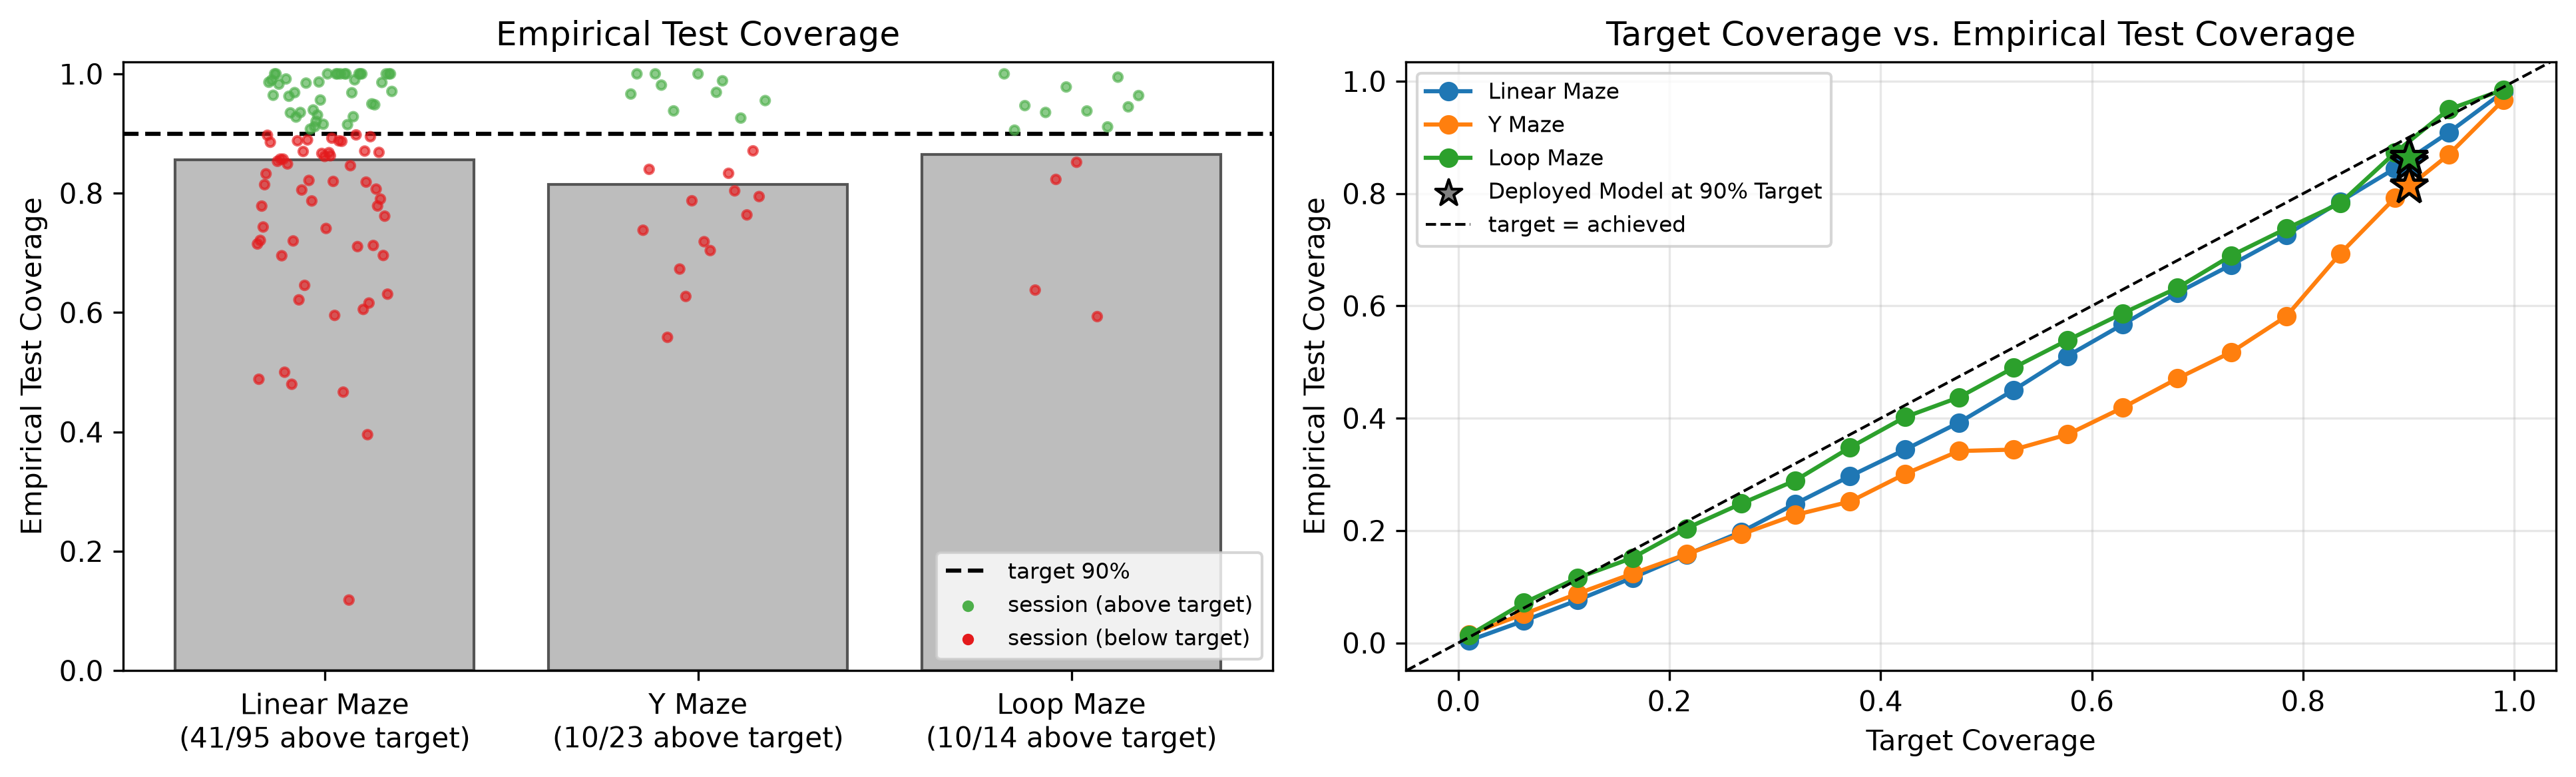
\includegraphics[width=\linewidth]{coverage-drift-tax.png}
  \caption{Calibration performance on test data. Left: Empirical test coverage per maze against the 90\% target, with sessions as points displaying the spread per maze. Right: Achieved test coverage after retraining the conformal layer for 20 coverage targets, equally distributed from 1\% to 99\%. The gap below the diagonal shows the empirical calibration cost between the validation set and the later test data.}
  \label{fig:coverage}
\end{figure}

\subsection{Coverage-sharpness trade-off}
\label{sec:trade-off}
Figure~\ref{fig:operating-curve} shows the frontier between coverage and sharpness obtained by retraining the conformal layer for 20 coverage targets, equally distributed from 1\% to 99\%. The horizontal axis reports achieved test coverage, while the vertical axis reports the mean trust region size normalized by the total number of maze regions. Higher achieved coverage is associated with larger trust regions, showing the expected trade-off.

The Linear Maze arguably has the best conformal performance, as identified by the lowest frontier, with a lower normalized trust region size for any given achieved coverage when compared with the Y and Loop Mazes. The Y and Loop Mazes require broader trust regions, consistent with their lower decoder accuracy and smaller datasets. The stars show the deployed models at a 90\% target, reported in Table~\ref{tab:results}.

\begin{figure}[t]
  \centering
  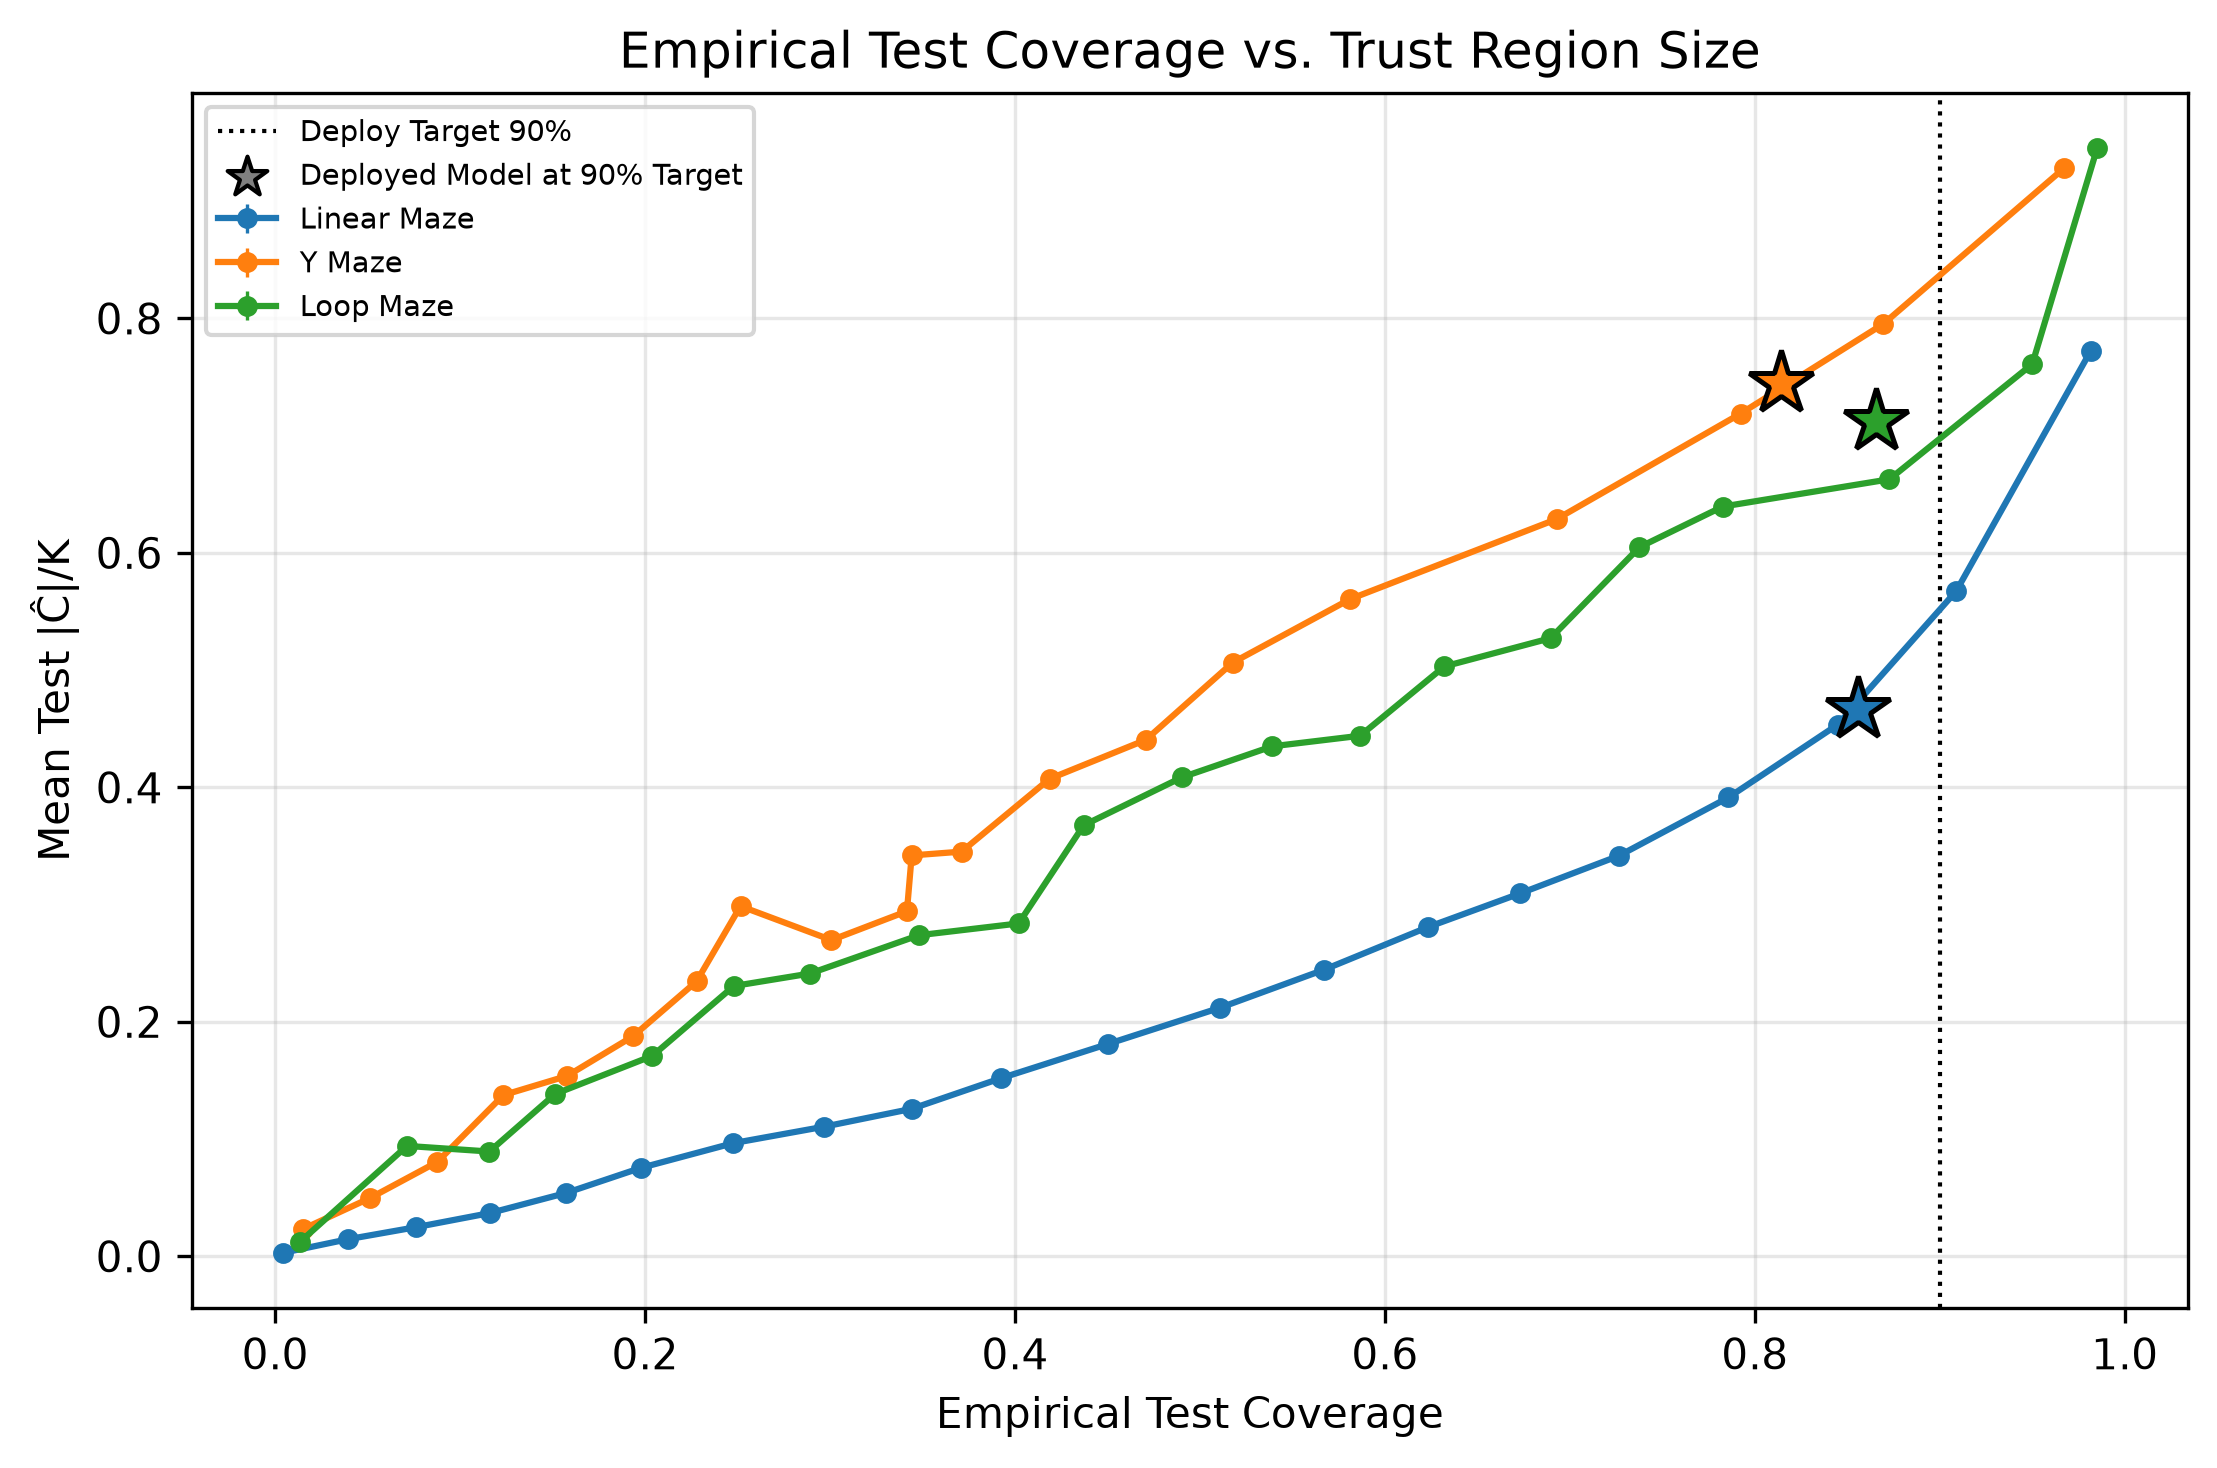
\includegraphics[width=0.7\linewidth]{coverage-sharpness-frontier.png}
  \caption{Coverage-sharpness trade-off. Achieved test coverage is shown on the horizontal axis, and mean trust region size normalized by total maze region count is shown on the vertical axis. Each curve retrains the conformal layer from scratch for 20 coverage targets, equally distributed from 1\% to 99\%. The star marks the deployed 90\% target models reported in Table~\ref{tab:results}.}
  \label{fig:operating-curve}
\end{figure}

\subsection{Class-conditional conformal performance}
Figure~\ref{fig:per-region} examines the conformal performance separately for each maze region. This analysis is important because the dataset's labels are highly imbalanced, so averages across the entire maze can mask weak behavior in rare regions. For each maze, the figure reports empirical test coverage, mean normalized trust region size, and the region's share of data points from the entire dataset.

The results per region show that test coverage differs across maze regions and should be interpreted alongside the mean trust region size. Some regions approach or exceed the 90\% coverage target, while others fall below it. The dataset share bars provide context for these differences, since regions with fewer data points tend to have worse conformal performance. In the Loop Maze, region 5 has no empirical test coverage or trust region size results because it had no test data points.

\begin{figure}[t]
  \centering
  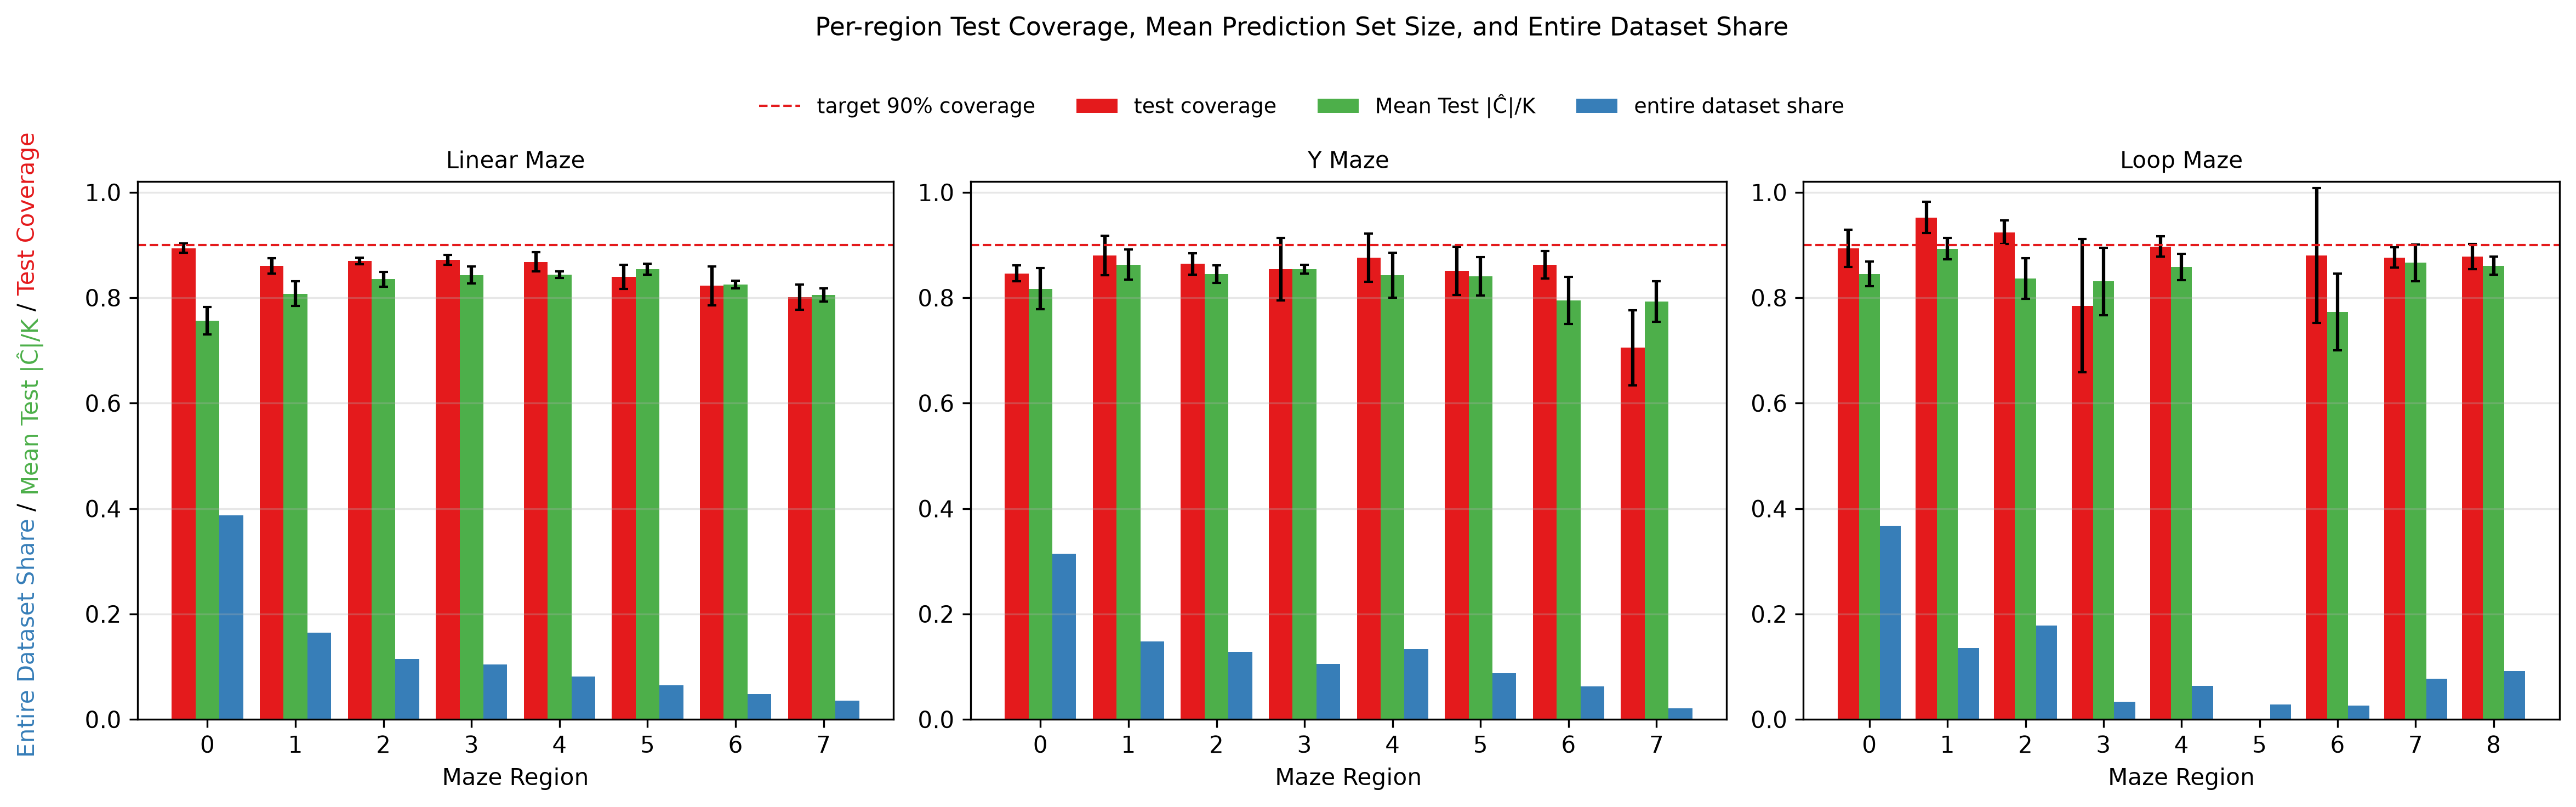
\includegraphics[width=\linewidth]{per-region-coverage.png}
  \caption{Conformal performance per region and label distribution. Each subplot corresponds to one maze. For inputs whose true label is the corresponding maze region, red bars show empirical test coverage, and green bars show the mean trust region size normalized by the number of maze regions. Blue bars show the region's share of data points for the entire dataset. The dashed line marks the 90\% coverage target. Region 5 in the Loop Maze has no test coverage or trust region size estimate because no test data points were present in that region.}
  \label{fig:per-region}
\end{figure}

\subsection{Decoder error correlations}
Table~\ref{tab:within-chunk} reports the Pearson correlation of test decoder error with the normalized trust region size and the learned uncertainty scale $\sigma_\theta(x)$. Decoder error is 0 or 1 for a single data point, so test data points are first grouped, as described in the caption, and each group contributes its error rate. Positive correlations indicate that the conformal layer produces a higher $\sigma_\theta(x)$ and creates larger trust regions where the decoder errs more often.

The Linear Maze shows strong positive correlations, 0.86 for trust region size and 0.99 for the learned scale. The Y Maze shows weaker positive correlations. In the Loop Maze both correlations are negative: the decoder errs more often where the trust regions are smaller, so there the conformal layer does not track decoder error.

\begin{table}[t]
  \caption{Decoder error Pearson correlations over grouped test data points. The first correlation groups by normalized trust region size $|\widehat{\mathcal{C}}|/K$, one group per size level. The second groups by the MLP uncertainty scale $\sigma_\theta(x)$, in 10 equal-count bins. Each group contributes its error rate and is weighted by its number of data points. Positive values indicate that decoder errors tend to coincide with larger trust regions or larger MLP scales.}
  \label{tab:within-chunk}
  \centering\footnotesize
  \begin{tabular}{@{}l c c@{}}
    \toprule
    Maze
    & corr(decoder error, $|\widehat{\mathcal{C}}|/K$)
    & corr(decoder error, $\sigma_\theta(x)$) \\
    \midrule
    Linear Maze & $+0.86$ & $+0.99$ \\
    Y Maze       & $+0.61$ & $+0.68$ \\
    Loop Maze    & $-0.78$ & $-0.86$ \\
    \bottomrule
  \end{tabular}
\end{table}

\subsection{Uncertainty signals contribution}
Figure~\ref{fig:signal-confound} shows how sensitive the MLP scale $\sigma_\theta(x)$ is to each one of the four uncertainty signals. Entropy shows the greatest sensitivity across all 3 mazes, indicating that the MLP relies more on the decoder's output. This is expected because predictive entropy is computed directly from the final softmax probability distribution.

However, the remaining signals also show comparable sensitivity, suggesting that $\sigma_\theta(x)$ is not exclusively determined by the entropy. Posterior variance is the second largest signal in the Linear Maze, and in the Y Maze is the alignment Jacobian. Loop Maze shows a more even contribution across posterior variance and both Jacobian signals.

\begin{figure}[t]
  \centering
  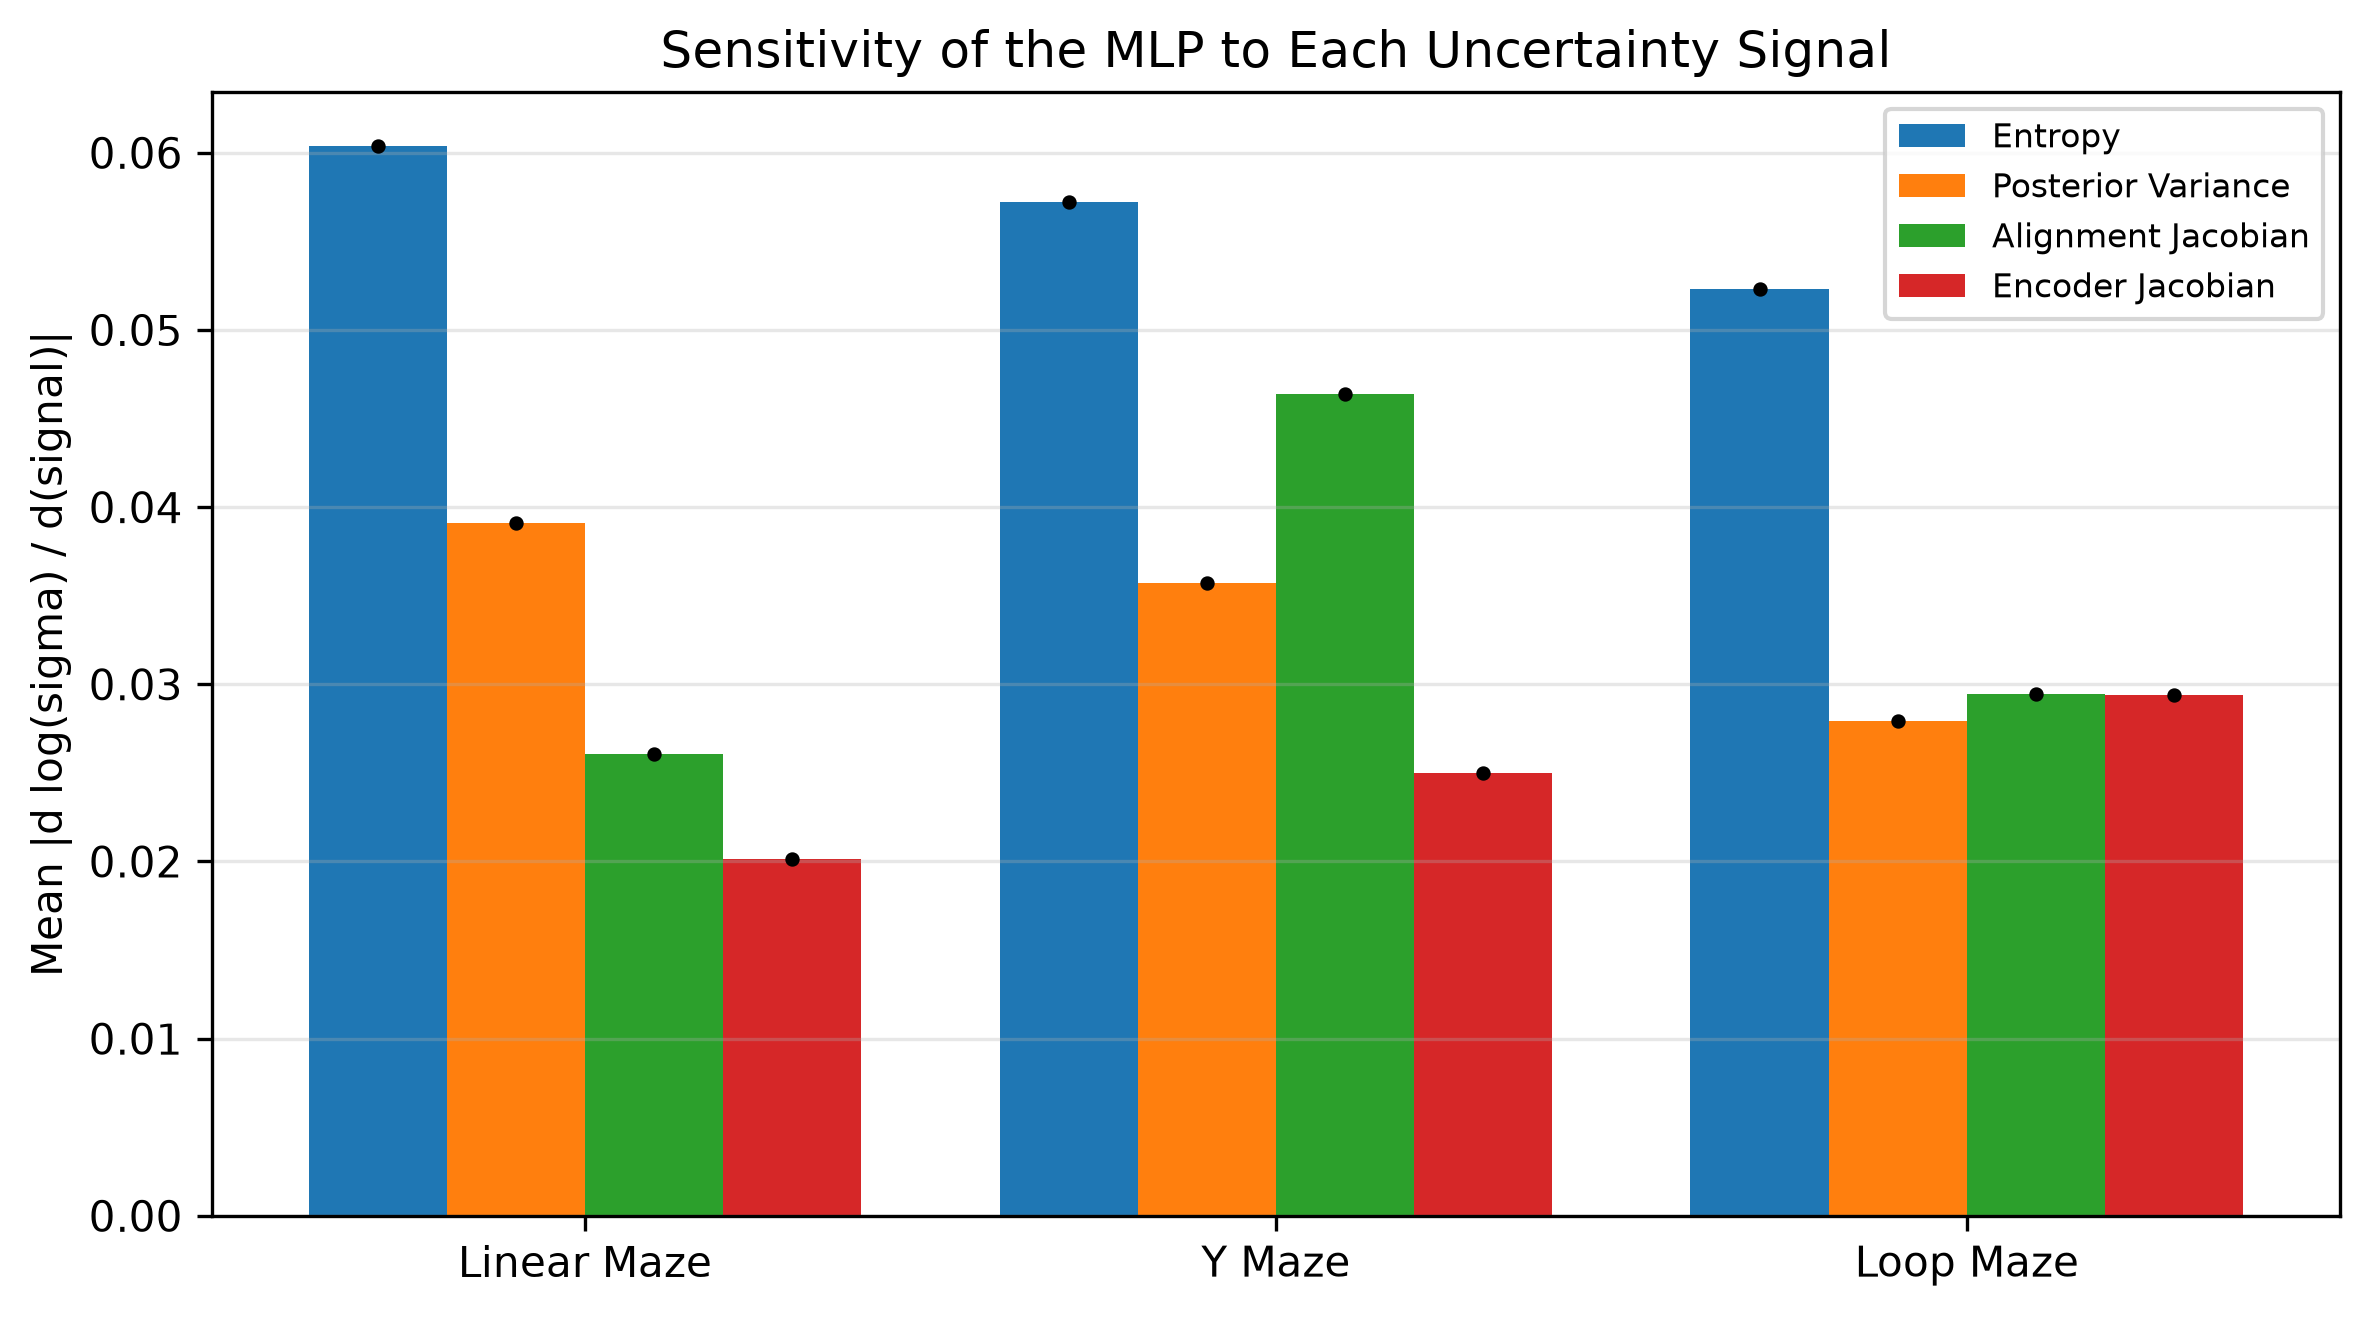
\includegraphics[width=0.7\linewidth]{signal-confound.png}
  \caption{Sensitivity of the learned conformal scale to each uncertainty signal. Bars show the mean relative change of $\sigma_\theta(x)$, $|\partial \log \sigma_\theta(x) / \partial z|$, per standard deviation $z$ of each input uncertainty signal, averaged over the test set for each maze. The relative change does not depend on the overall level of $\sigma_\theta(x)$, so the mazes can be compared directly.}
  \label{fig:signal-confound}
\end{figure}

\section{Discussion}
The results show that the conformal layer can construct a trust region that retains a substantial empirical coverage around the predictions of a low accuracy decoder. The coverage is obtained at the cost of larger trust regions due to the decoder's low performance. Indicating that the conformal layer is serving its design purpose and analyzing the encoding-decoding pipeline uncertainty to output wider trust regions, converting what could otherwise be mistrusted predictions into a quantifiable reliability metric.

\subsection{Conformal calibration}
Across all 3 mazes, the conformal layer retained substantial empirical coverage, but coverage did not precisely match the 90\% target. This gap reflects the cost of applying a split-conformal method to neural data. Where the final thresholds were calibrated on the validation data and conformal performance is measured on the test set. In this paper, that gap is treated as a split-conformal calibration cost, called the drift tax, due to the neural drift's impact on the dataset used.

The test coverage spread across sessions indicates that the drift tax is not uniform across recordings. Moreover, the drift tax shows that the coverage target should not be interpreted as the expected empirical coverage in neural data. If a BCI application requires a specific empirical coverage level, the requested target should be set higher to account for this gap. However, setting a higher target also widens the trust regions, reducing sharpness. As shown by the coverage and sharpness trade-off, higher coverage can be achieved, but at the cost of less informative trust regions.

\subsection{Decoder performance}
The results show that decoder performance directly translates to conformal layer performance. The Linear Maze has the highest decoder accuracy, producing the sharpest trust regions and the lowest coverage and sharpness curve. Whereas the Y and Loop Mazes have lower decoder accuracy and require broader trust regions to maintain coverage. This is consistent with the intended role of the conformal layer, as it's not designed to correct decoder errors, but to express lower confidence by returning wider trust regions.

When the encoding-decoding pipeline uncertainty signals indicate high distrust, the conformal layer has no other option but to create wider trust regions to avoid sacrificing coverage. Therefore, the decoder accuracy limits how sharp the trust regions can be. The different results in trust region sharpness across mazes, along with the positive correlations of decoder error with trust region size and the MLP output in the Linear and Y Mazes, support the interpretation that the conformal layer tracks decoder uncertainty in those mazes. In the Loop Maze the correlations are negative, so there the conformal layer does not track decoder error.

\subsection{Classes imbalance}
The analysis per region in Figure~\ref{fig:per-region} shows why a class-conditional conformal method is important for imbalanced datasets. The data used in this paper has a highly imbalanced label distribution. Not using a class-conditional approach would mean using a single conformal threshold, so conformal scores would not be stored per maze region. In this case, a single threshold would set the rule for the entire maze, determining which regions to include in the trust region.

In contrast, the class-conditional method applied calibrates separate thresholds for each maze region. With this approach, the results show that, even though regions with less data still suffer, conformal performance remains balanced within tolerance throughout the maze, especially taking into consideration how imbalanced the label distribution is. This is possible because, in maze regions with less data, coverage is usually achieved using wider trust regions.

Nevertheless, a stricter comparison between a class-conditional and a regular conformal method under the same conditions is needed to draw stronger conclusions.

\subsection{Signals Contributions}
The MLP output, the learned scale, is most sensitive to the predictive entropy uncertainty signal for all 3 mazes. This is expected since entropy is computed directly from the decoder’s final probability softmax distribution over the maze regions. Nevertheless, the posterior variance and the Jacobian signals also contribute. These results support all the uncertainty diagnostic signals computed for the encoding-decoding pipeline. However, further analysis is needed to prove that they are all strictly necessary to achieve the displayed conformal performance.

\subsection{Limitations and future work}
The main limitation of this study is the limited size and imbalance of the available dataset. This constraint affects both the encoder-decoder and the conformal layer, especially in the Y and Loop Mazes. The Loop Maze is the clearest example because it has only two mice available, decoder accuracy was the lowest, and maze region 5 had no test data.

The data from all available mice was aggregated within each maze to increase the number of available data points. This approach supports the present analysis, but prevents strong conclusions about performance within individual mice, across sessions, or across animals. Subsequent work should evaluate the conformal layer under stricter animal and session data splits once enough data is available. In the meantime, artificially generated neural data could also be used.

The present analysis does not yet include the comparisons needed to isolate the contribution of each design choice. Upcoming research should compare the MLP scale against a standard conformal approach with $\sigma_\theta(x)=1$, and compare class-conditional thresholds against a single threshold. Furthermore, future work should also test the conformal layer approach with other encoding-decoding architectures~\cite{schneider2023a,azabou2023}. Experiments are also needed to determine whether the posterior variance and the Jacobian uncertainty signals improve performance beyond predictive entropy alone. Additional new uncertainty signals could also be implemented and paired with temporally structured models, such as recurrent neural networks, rather than an MLP.

Finally, the current task is limited to discrete classification. With bigger datasets and stronger decoder performance, the conformal layer could be extended towards continuous position decoding, where the trust region would correspond to a continuous spatial region rather than a set of discrete labels~\cite{angelopoulos2022a}, possibly resulting in a much more informative reliability metric to quantify the impact of neural drift in BCI applications.

\section{Conclusion}
This paper evaluated a learned class-conditional split-conformal layer for uncertainty-aware neural decoding under neural drift. The method was applied after a BC-VAE and a Transformer decoder, creating trust regions of plausible results for neural decoding. Across 3 virtual-reality maze navigation experiments recorded from flexible brain probes, the conformal layer retained substantial empirical coverage on unseen data.

The main finding is that the conformal layer provides reliability information regarding the current decoder performance without requiring recent labeled data. When the decoder performance was weaker, the trust regions became broader, indicating that the method autonomously identified greater uncertainty in the encoding-decoding pipeline. Proving that the proposed model could serve as a prospective reliability layer for BCI decoding pipelines, which is highly needed for the viability of chronic BCIs under neural drift. However, wider implementation of the presented method still depends on larger dataset experiments and comparisons against baseline methods.

\section*{Data Availability}
The data used in this paper is owned by the Liu Lab for Bioelectronics at the Harvard John A. Paulson School of Engineering and Applied Sciences. Database access instructions are available at \url{https://github.com/ese-ada-lovelace-2025/irp-ggf25}, but access requires private credentials.

\section*{Code Availability and Reproducibility}
The code used to perform the paper’s analyses is available at \url{https://github.com/ese-ada-lovelace-2025/irp-ggf25}. A fixed random seed of 42 was used throughout. Unless otherwise stated in their respective captions, the final figures and tables were generated using the notebook at \url{https://github.com/ese-ada-lovelace-2025/irp-ggf25/blob/main/analyses/cross_maze.ipynb}.

\section*{AI Acknowledgments}
I acknowledge using ChatGPT (model: GPT‑5.6) by OpenAI (\url{https://openai.com/chatgpt}) and Claude (model: Sonnet 4.8) by Anthropic (\url{https://claude.ai/}) to support drafting code documentation and code tests, debugging code, and brainstorming code implementation choices. I used the GitLens extension for Visual Studio (\url{https://gitlens.amod.io}) together with GitHub Copilot (\url{https://github.com/features/copilot}) to help phrase commit messages and pull request descriptions. I confirm that the work submitted is my own and that I verified and adapted all AI outputs.

\begin{ack}
I thank Professor Jia Liu for the opportunity to conduct this project in the Liu Lab and for his guidance. I am grateful to Dr. Tom Davison for his supervision, and to Hao Shen and Tianshu Tan for their support. I also thank the rest of the Liu Lab members for their insightful discussions throughout the project.
\end{ack}

\bibliographystyle{unsrtnat}
\bibliography{references}

% The NeurIPS paper checklist is mandatory for submission; it does not count toward the page limit.
\section*{NeurIPS Paper Checklist}

%%% BEGIN INSTRUCTIONS %%%
The checklist is designed to encourage best practices for responsible machine learning research, addressing issues of reproducibility, transparency, research ethics, and societal impact. Do not remove the checklist: {\bf The papers not including the checklist will be desk rejected.} The checklist should follow the references and follow the (optional) supplemental material.  The checklist does NOT count towards the page
limit. 

Please read the checklist guidelines carefully for information on how to answer these questions. For each question in the checklist:
\begin{itemize}
    \item You should answer \answerYes{}, \answerNo{}, or \answerNA{}.
    \item \answerNA{} means either that the question is Not Applicable for that particular paper or the relevant information is Not Available.
    \item Please provide a short (1--2 sentence) justification right after your answer (even for \answerNA). 
   % \item {\bf The papers not including the checklist will be desk rejected.}
\end{itemize}

{\bf The checklist answers are an integral part of your paper submission.} They are visible to the reviewers, area chairs, senior area chairs, and ethics reviewers. You will also be asked to include it (after eventual revisions) with the final version of your paper, and its final version will be published with the paper.

The reviewers of your paper will be asked to use the checklist as one of the factors in their evaluation. While \answerYes{} is generally preferable to \answerNo{}, it is perfectly acceptable to answer \answerNo{} provided a proper justification is given (e.g., error bars are not reported because it would be too computationally expensive'' or ``we were unable to find the license for the dataset we used''). In general, answering \answerNo{} or \answerNA{} is not grounds for rejection. While the questions are phrased in a binary way, we acknowledge that the true answer is often more nuanced, so please just use your best judgment and write a justification to elaborate. All supporting evidence can appear either in the main paper or the supplemental material, provided in appendix. If you answer \answerYes{} to a question, in the justification please point to the section(s) where related material for the question can be found.

IMPORTANT, please:
\begin{itemize}
    \item {\bf Delete this instruction block, but keep the section heading ``NeurIPS Paper Checklist"},
    \item  {\bf Keep the checklist subsection headings, questions/answers and guidelines below.}
    \item {\bf Do not modify the questions and only use the provided macros for your answers}.
\end{itemize} 
 

%%% END INSTRUCTIONS %%%


\begin{enumerate}

\item {\bf Claims}
    \item[] Question: Do the main claims made in the abstract and introduction accurately reflect the paper's contributions and scope?
    \item[] Answer: \answerTODO{} % Replace by \answerYes{}, \answerNo{}, or \answerNA{}.
    \item[] Justification: \justificationTODO{}
    \item[] Guidelines:
    \begin{itemize}
        \item The answer \answerNA{} means that the abstract and introduction do not include the claims made in the paper.
        \item The abstract and/or introduction should clearly state the claims made, including the contributions made in the paper and important assumptions and limitations. A \answerNo{} or \answerNA{} answer to this question will not be perceived well by the reviewers. 
        \item The claims made should match theoretical and experimental results, and reflect how much the results can be expected to generalize to other settings. 
        \item It is fine to include aspirational goals as motivation as long as it is clear that these goals are not attained by the paper. 
    \end{itemize}

\item {\bf Limitations}
    \item[] Question: Does the paper discuss the limitations of the work performed by the authors?
    \item[] Answer: \answerTODO{} % Replace by \answerYes{}, \answerNo{}, or \answerNA{}.
    \item[] Justification: \justificationTODO{}
    \item[] Guidelines:
    \begin{itemize}
        \item The answer \answerNA{} means that the paper has no limitation while the answer \answerNo{} means that the paper has limitations, but those are not discussed in the paper. 
        \item The authors are encouraged to create a separate ``Limitations'' section in their paper.
        \item The paper should point out any strong assumptions and how robust the results are to violations of these assumptions (e.g., independence assumptions, noiseless settings, model well-specification, asymptotic approximations only holding locally). The authors should reflect on how these assumptions might be violated in practice and what the implications would be.
        \item The authors should reflect on the scope of the claims made, e.g., if the approach was only tested on a few datasets or with a few runs. In general, empirical results often depend on implicit assumptions, which should be articulated.
        \item The authors should reflect on the factors that influence the performance of the approach. For example, a facial recognition algorithm may perform poorly when image resolution is low or images are taken in low lighting. Or a speech-to-text system might not be used reliably to provide closed captions for online lectures because it fails to handle technical jargon.
        \item The authors should discuss the computational efficiency of the proposed algorithms and how they scale with dataset size.
        \item If applicable, the authors should discuss possible limitations of their approach to address problems of privacy and fairness.
        \item While the authors might fear that complete honesty about limitations might be used by reviewers as grounds for rejection, a worse outcome might be that reviewers discover limitations that aren't acknowledged in the paper. The authors should use their best judgment and recognize that individual actions in favor of transparency play an important role in developing norms that preserve the integrity of the community. Reviewers will be specifically instructed to not penalize honesty concerning limitations.
    \end{itemize}

\item {\bf Theory assumptions and proofs}
    \item[] Question: For each theoretical result, does the paper provide the full set of assumptions and a complete (and correct) proof?
    \item[] Answer: \answerTODO{} % Replace by \answerYes{}, \answerNo{}, or \answerNA{}.
    \item[] Justification: \justificationTODO{}
    \item[] Guidelines:
    \begin{itemize}
        \item The answer \answerNA{} means that the paper does not include theoretical results. 
        \item All the theorems, formulas, and proofs in the paper should be numbered and cross-referenced.
        \item All assumptions should be clearly stated or referenced in the statement of any theorems.
        \item The proofs can either appear in the main paper or the supplemental material, but if they appear in the supplemental material, the authors are encouraged to provide a short proof sketch to provide intuition. 
        \item Inversely, any informal proof provided in the core of the paper should be complemented by formal proofs provided in appendix or supplemental material.
        \item Theorems and Lemmas that the proof relies upon should be properly referenced. 
    \end{itemize}

    \item {\bf Experimental result reproducibility}
    \item[] Question: Does the paper fully disclose all the information needed to reproduce the main experimental results of the paper to the extent that it affects the main claims and/or conclusions of the paper (regardless of whether the code and data are provided or not)?
    \item[] Answer: \answerTODO{} % Replace by \answerYes{}, \answerNo{}, or \answerNA{}.
    \item[] Justification: \justificationTODO{}
    \item[] Guidelines:
    \begin{itemize}
        \item The answer \answerNA{} means that the paper does not include experiments.
        \item If the paper includes experiments, a \answerNo{} answer to this question will not be perceived well by the reviewers: Making the paper reproducible is important, regardless of whether the code and data are provided or not.
        \item If the contribution is a dataset and\slash or model, the authors should describe the steps taken to make their results reproducible or verifiable. 
        \item Depending on the contribution, reproducibility can be accomplished in various ways. For example, if the contribution is a novel architecture, describing the architecture fully might suffice, or if the contribution is a specific model and empirical evaluation, it may be necessary to either make it possible for others to replicate the model with the same dataset, or provide access to the model. In general. releasing code and data is often one good way to accomplish this, but reproducibility can also be provided via detailed instructions for how to replicate the results, access to a hosted model (e.g., in the case of a large language model), releasing of a model checkpoint, or other means that are appropriate to the research performed.
        \item While NeurIPS does not require releasing code, the conference does require all submissions to provide some reasonable avenue for reproducibility, which may depend on the nature of the contribution. For example
        \begin{enumerate}
            \item If the contribution is primarily a new algorithm, the paper should make it clear how to reproduce that algorithm.
            \item If the contribution is primarily a new model architecture, the paper should describe the architecture clearly and fully.
            \item If the contribution is a new model (e.g., a large language model), then there should either be a way to access this model for reproducing the results or a way to reproduce the model (e.g., with an open-source dataset or instructions for how to construct the dataset).
            \item We recognize that reproducibility may be tricky in some cases, in which case authors are welcome to describe the particular way they provide for reproducibility. In the case of closed-source models, it may be that access to the model is limited in some way (e.g., to registered users), but it should be possible for other researchers to have some path to reproducing or verifying the results.
        \end{enumerate}
    \end{itemize}


\item {\bf Open access to data and code}
    \item[] Question: Does the paper provide open access to the data and code, with sufficient instructions to faithfully reproduce the main experimental results, as described in supplemental material?
    \item[] Answer: \answerTODO{} % Replace by \answerYes{}, \answerNo{}, or \answerNA{}.
    \item[] Justification: \justificationTODO{}
    \item[] Guidelines:
    \begin{itemize}
        \item The answer \answerNA{} means that paper does not include experiments requiring code.
        \item Please see the NeurIPS code and data submission guidelines (\url{https://neurips.cc/public/guides/CodeSubmissionPolicy}) for more details.
        \item While we encourage the release of code and data, we understand that this might not be possible, so \answerNo{} is an acceptable answer. Papers cannot be rejected simply for not including code, unless this is central to the contribution (e.g., for a new open-source benchmark).
        \item The instructions should contain the exact command and environment needed to run to reproduce the results. See the NeurIPS code and data submission guidelines (\url{https://neurips.cc/public/guides/CodeSubmissionPolicy}) for more details.
        \item The authors should provide instructions on data access and preparation, including how to access the raw data, preprocessed data, intermediate data, and generated data, etc.
        \item The authors should provide scripts to reproduce all experimental results for the new proposed method and baselines. If only a subset of experiments are reproducible, they should state which ones are omitted from the script and why.
        \item At submission time, to preserve anonymity, the authors should release anonymized versions (if applicable).
        \item Providing as much information as possible in supplemental material (appended to the paper) is recommended, but including URLs to data and code is permitted.
    \end{itemize}


\item {\bf Experimental setting/details}
    \item[] Question: Does the paper specify all the training and test details (e.g., data splits, hyperparameters, how they were chosen, type of optimizer) necessary to understand the results?
    \item[] Answer: \answerTODO{} % Replace by \answerYes{}, \answerNo{}, or \answerNA{}.
    \item[] Justification: \justificationTODO{}
    \item[] Guidelines:
    \begin{itemize}
        \item The answer \answerNA{} means that the paper does not include experiments.
        \item The experimental setting should be presented in the core of the paper to a level of detail that is necessary to appreciate the results and make sense of them.
        \item The full details can be provided either with the code, in appendix, or as supplemental material.
    \end{itemize}

\item {\bf Experiment statistical significance}
    \item[] Question: Does the paper report error bars suitably and correctly defined or other appropriate information about the statistical significance of the experiments?
    \item[] Answer: \answerTODO{} % Replace by \answerYes{}, \answerNo{}, or \answerNA{}.
    \item[] Justification: \justificationTODO{}
    \item[] Guidelines:
    \begin{itemize}
        \item The answer \answerNA{} means that the paper does not include experiments.
        \item The authors should answer \answerYes{} if the results are accompanied by error bars, confidence intervals, or statistical significance tests, at least for the experiments that support the main claims of the paper.
        \item The factors of variability that the error bars are capturing should be clearly stated (for example, train/test split, initialization, random drawing of some parameter, or overall run with given experimental conditions).
        \item The method for calculating the error bars should be explained (closed form formula, call to a library function, bootstrap, etc.)
        \item The assumptions made should be given (e.g., Normally distributed errors).
        \item It should be clear whether the error bar is the standard deviation or the standard error of the mean.
        \item It is OK to report 1-sigma error bars, but one should state it. The authors should preferably report a 2-sigma error bar than state that they have a 96\% CI, if the hypothesis of Normality of errors is not verified.
        \item For asymmetric distributions, the authors should be careful not to show in tables or figures symmetric error bars that would yield results that are out of range (e.g., negative error rates).
        \item If error bars are reported in tables or plots, the authors should explain in the text how they were calculated and reference the corresponding figures or tables in the text.
    \end{itemize}

\item {\bf Experiments compute resources}
    \item[] Question: For each experiment, does the paper provide sufficient information on the computer resources (type of compute workers, memory, time of execution) needed to reproduce the experiments?
    \item[] Answer: \answerTODO{} % Replace by \answerYes{}, \answerNo{}, or \answerNA{}.
    \item[] Justification: \justificationTODO{}
    \item[] Guidelines:
    \begin{itemize}
        \item The answer \answerNA{} means that the paper does not include experiments.
        \item The paper should indicate the type of compute workers CPU or GPU, internal cluster, or cloud provider, including relevant memory and storage.
        \item The paper should provide the amount of compute required for each of the individual experimental runs as well as estimate the total compute. 
        \item The paper should disclose whether the full research project required more compute than the experiments reported in the paper (e.g., preliminary or failed experiments that didn't make it into the paper). 
    \end{itemize}
    
\item {\bf Code of ethics}
    \item[] Question: Does the research conducted in the paper conform, in every respect, with the NeurIPS Code of Ethics \url{https://neurips.cc/public/EthicsGuidelines}?
    \item[] Answer: \answerTODO{} % Replace by \answerYes{}, \answerNo{}, or \answerNA{}.
    \item[] Justification: \justificationTODO{}
    \item[] Guidelines:
    \begin{itemize}
        \item The answer \answerNA{} means that the authors have not reviewed the NeurIPS Code of Ethics.
        \item If the authors answer \answerNo, they should explain the special circumstances that require a deviation from the Code of Ethics.
        \item The authors should make sure to preserve anonymity (e.g., if there is a special consideration due to laws or regulations in their jurisdiction).
    \end{itemize}


\item {\bf Broader impacts}
    \item[] Question: Does the paper discuss both potential positive societal impacts and negative societal impacts of the work performed?
    \item[] Answer: \answerTODO{} % Replace by \answerYes{}, \answerNo{}, or \answerNA{}.
    \item[] Justification: \justificationTODO{}
    \item[] Guidelines:
    \begin{itemize}
        \item The answer \answerNA{} means that there is no societal impact of the work performed.
        \item If the authors answer \answerNA{} or \answerNo, they should explain why their work has no societal impact or why the paper does not address societal impact.
        \item Examples of negative societal impacts include potential malicious or unintended uses (e.g., disinformation, generating fake profiles, surveillance), fairness considerations (e.g., deployment of technologies that could make decisions that unfairly impact specific groups), privacy considerations, and security considerations.
        \item The conference expects that many papers will be foundational research and not tied to particular applications, let alone deployments. However, if there is a direct path to any negative applications, the authors should point it out. For example, it is legitimate to point out that an improvement in the quality of generative models could be used to generate Deepfakes for disinformation. On the other hand, it is not needed to point out that a generic algorithm for optimizing neural networks could enable people to train models that generate Deepfakes faster.
        \item The authors should consider possible harms that could arise when the technology is being used as intended and functioning correctly, harms that could arise when the technology is being used as intended but gives incorrect results, and harms following from (intentional or unintentional) misuse of the technology.
        \item If there are negative societal impacts, the authors could also discuss possible mitigation strategies (e.g., gated release of models, providing defenses in addition to attacks, mechanisms for monitoring misuse, mechanisms to monitor how a system learns from feedback over time, improving the efficiency and accessibility of ML).
    \end{itemize}
    
\item {\bf Safeguards}
    \item[] Question: Does the paper describe safeguards that have been put in place for responsible release of data or models that have a high risk for misuse (e.g., pre-trained language models, image generators, or scraped datasets)?
    \item[] Answer: \answerTODO{} % Replace by \answerYes{}, \answerNo{}, or \answerNA{}.
    \item[] Justification: \justificationTODO{}
    \item[] Guidelines:
    \begin{itemize}
        \item The answer \answerNA{} means that the paper poses no such risks.
        \item Released models that have a high risk for misuse or dual-use should be released with necessary safeguards to allow for controlled use of the model, for example by requiring that users adhere to usage guidelines or restrictions to access the model or implementing safety filters. 
        \item Datasets that have been scraped from the Internet could pose safety risks. The authors should describe how they avoided releasing unsafe images.
        \item We recognize that providing effective safeguards is challenging, and many papers do not require this, but we encourage authors to take this into account and make a best faith effort.
    \end{itemize}

\item {\bf Licenses for existing assets}
    \item[] Question: Are the creators or original owners of assets (e.g., code, data, models), used in the paper, properly credited and are the license and terms of use explicitly mentioned and properly respected?
    \item[] Answer: \answerTODO{} % Replace by \answerYes{}, \answerNo{}, or \answerNA{}.
    \item[] Justification: \justificationTODO{}
    \item[] Guidelines:
    \begin{itemize}
        \item The answer \answerNA{} means that the paper does not use existing assets.
        \item The authors should cite the original paper that produced the code package or dataset.
        \item The authors should state which version of the asset is used and, if possible, include a URL.
        \item The name of the license (e.g., CC-BY 4.0) should be included for each asset.
        \item For scraped data from a particular source (e.g., website), the copyright and terms of service of that source should be provided.
        \item If assets are released, the license, copyright information, and terms of use in the package should be provided. For popular datasets, \url{paperswithcode.com/datasets} has curated licenses for some datasets. Their licensing guide can help determine the license of a dataset.
        \item For existing datasets that are re-packaged, both the original license and the license of the derived asset (if it has changed) should be provided.
        \item If this information is not available online, the authors are encouraged to reach out to the asset's creators.
    \end{itemize}

\item {\bf New assets}
    \item[] Question: Are new assets introduced in the paper well documented and is the documentation provided alongside the assets?
    \item[] Answer: \answerTODO{} % Replace by \answerYes{}, \answerNo{}, or \answerNA{}.
    \item[] Justification: \justificationTODO{}
    \item[] Guidelines:
    \begin{itemize}
        \item The answer \answerNA{} means that the paper does not release new assets.
        \item Researchers should communicate the details of the dataset\slash code\slash model as part of their submissions via structured templates. This includes details about training, license, limitations, etc. 
        \item The paper should discuss whether and how consent was obtained from people whose asset is used.
        \item At submission time, remember to anonymize your assets (if applicable). You can either create an anonymized URL or include an anonymized zip file.
    \end{itemize}

\item {\bf Crowdsourcing and research with human subjects}
    \item[] Question: For crowdsourcing experiments and research with human subjects, does the paper include the full text of instructions given to participants and screenshots, if applicable, as well as details about compensation (if any)? 
    \item[] Answer: \answerTODO{} % Replace by \answerYes{}, \answerNo{}, or \answerNA{}.
    \item[] Justification: \justificationTODO{}
    \item[] Guidelines:
    \begin{itemize}
        \item The answer \answerNA{} means that the paper does not involve crowdsourcing nor research with human subjects.
        \item Including this information in the supplemental material is fine, but if the main contribution of the paper involves human subjects, then as much detail as possible should be included in the main paper. 
        \item According to the NeurIPS Code of Ethics, workers involved in data collection, curation, or other labor should be paid at least the minimum wage in the country of the data collector. 
    \end{itemize}

\item {\bf Institutional review board (IRB) approvals or equivalent for research with human subjects}
    \item[] Question: Does the paper describe potential risks incurred by study participants, whether such risks were disclosed to the subjects, and whether Institutional Review Board (IRB) approvals (or an equivalent approval/review based on the requirements of your country or institution) were obtained?
    \item[] Answer: \answerTODO{} % Replace by \answerYes{}, \answerNo{}, or \answerNA{}.
    \item[] Justification: \justificationTODO{}
    \item[] Guidelines:
    \begin{itemize}
        \item The answer \answerNA{} means that the paper does not involve crowdsourcing nor research with human subjects.
        \item Depending on the country in which research is conducted, IRB approval (or equivalent) may be required for any human subjects research. If you obtained IRB approval, you should clearly state this in the paper. 
        \item We recognize that the procedures for this may vary significantly between institutions and locations, and we expect authors to adhere to the NeurIPS Code of Ethics and the guidelines for their institution. 
        \item For initial submissions, do not include any information that would break anonymity (if applicable), such as the institution conducting the review.
    \end{itemize}

\item {\bf Declaration of LLM usage}
    \item[] Question: Does the paper describe the usage of LLMs if it is an important, original, or non-standard component of the core methods in this research? Note that if the LLM is used only for writing, editing, or formatting purposes and does \emph{not} impact the core methodology, scientific rigor, or originality of the research, declaration is not required.
    %this research? 
    \item[] Answer: \answerTODO{} % Replace by \answerYes{}, \answerNo{}, or \answerNA{}.
    \item[] Justification: \justificationTODO{}
    \item[] Guidelines:
    \begin{itemize}
        \item The answer \answerNA{} means that the core method development in this research does not involve LLMs as any important, original, or non-standard components.
        \item Please refer to our LLM policy in the NeurIPS handbook for what should or should not be described.
    \end{itemize}

\end{enumerate}

\end{document}
